%Gilmore Space LaTeX template
%
%Rory Kelly ~ 21 Nov 2024
%Needed for ?. Must come before document class
\RequirePackage{pdfmanagement-testphase}
\DeclareDocumentMetadata{}
\documentclass[12pt]{article}

% Page setup
\usepackage[a4paper]{geometry}

% PDF management (to include PDF pages)
\usepackage{pdfpages}

% Table management (for advanced table formatting)
\usepackage{tabu}

% Font handling
\usepackage{mathspec} 
%\usepackage[no-math]{fontspec} 
\usepackage{fontspec} % for font selection and OpenType/TrueType support

\usepackage[english]{babel} 

% Mathematics support
\usepackage{amsmath, amssymb, amsthm, thmtools}

%\usepackage[no-math]{fontspec} 
%\setmainfont{Gentium Plus} 
%\usepackage[italic]{mathastext}

% Input encoding
\usepackage[utf8]{inputenc}

% File-related commands (for working with file paths)
\usepackage[abspath]{currfile} 

% Section and subsection formatting
\usepackage{titlesec}

% Drawing and custom graphics
\usepackage{tikz} 

% Watermark management
\usepackage{eso-pic} 

% Header and footer formatting
\usepackage{fancyhdr} 

% Get total number of pages
\usepackage{lastpage}

% Optional package for total page count (not used here)
% \usepackage{zref-totpages} % gets the total page numbers

% Graphics support
\usepackage{graphicx}
\usepackage{float}
\usepackage{transparent} % for transparent watermark

% Hyperlink support
\usepackage[colorlinks, allcolors=blue]{hyperref}

% Table formatting
\usepackage{longtable}
\usepackage{booktabs}
\usepackage{adjustbox}
\usepackage{multirow}
\usepackage{multicol}
\usepackage{array}
\usepackage{tabularx}

% Color support
\usepackage[table, svgnames, dvipsnames]{xcolor}
\definecolor{lightbeige}{RGB}{255, 239, 204}
\definecolor{green}{RGB}{0, 128, 0}
\definecolor{codegreen}{rgb}{0, 0.6, 0}
\definecolor{codegray}{rgb}{0.5, 0.5, 0.5}
\definecolor{codepurple}{rgb}{0.58, 0, 0.82}
\definecolor{backcolour}{rgb}{0.95, 0.95, 0.92}

% Code formatting
\usepackage{verbatim}
\usepackage{listings}
\lstset{
    backgroundcolor=\color{backcolour},   
    commentstyle=\color{codegreen},
    keywordstyle=\color{magenta},
    numberstyle=\tiny\color{codegray},
    stringstyle=\color{codepurple},
    basicstyle=\ttfamily\footnotesize,
    breakatwhitespace=false,         
    breaklines=true,                 
    captionpos=b,                    
    keepspaces=true,                 
    numbers=left,                    
    numbersep=5pt,                  
    showspaces=false,                
    showstringspaces=false,
    showtabs=false,                  
    tabsize=2
}

% Caption setup for tables
\usepackage{caption}
\captionsetup[table]{skip=2pt}

% Additional useful packages
\usepackage{subfigure}  % for subfigures
\usepackage{lscape}     % for landscape pages
\usepackage{makecell}   % for table cells
\usepackage{rotating}   % for rotating elements
\usepackage{nomencl}    % for nomenclature

% Clever references
\usepackage[nameinlink, capitalize]{cleveref}

% Miscellaneous styling
\usepackage{color,soul}
%\usepackage{stix, bbm, pifont, utfsym, fontawesome, noto}
\usepackage{stix, bbm, pifont, fontawesome, noto}

\usepackage{ulem}

\setmainfont{Arial}[
]
%
\definecolor{AtmoBlue}{HTML}{00aeef}
\definecolor{DeepSpace}{HTML}{0c004b}
\definecolor{Rocket}{HTML}{c9cacc}
\definecolor{Titles}{HTML}{2f5496}
\definecolor{Table_Light}{HTML}{deeaf6}
\definecolor{Table_Dark}{HTML}{bdd6ee}
\definecolor{Table_Title}{HTML}{5b9bd5}
%
\titleformat{\section}
{\color{Titles}\normalfont\Large}
{\color{Titles}\thesection}{1em}{}
\titleformat{\subsection}
{\color{Titles}\normalfont\large}
{\color{Titles}\thesubsection}{1em}{}
\titleformat{\subsubsection}
{\color{Titles}\normalfont}
{\color{Titles}\thesubsubsection}{1em}{}
%
%%%%%%%%%%%%%%%%%%%%%%%%%%%%%%%%%%%%%%%%%%%%%%%%%%%%%%%%%%%%%%%%%%%%%%%
%%%%%%%%%%%%%%%%%%%%%%%%%%%%%%%%%%%%%%%%%%%%%%%%%%%%%%%%%%%%%%%%%%%%%%%
%%%%%%%%%%%%%%%%%%%%%%%%%%%%%%%%%%%%%%%%%%%%%%%%%%%%%%%%%%%%%%%%%%%%%%%
%
% IMPORTANT, PUT THE DOCUMENT INFORMATION HERE!!!
\newcommand{\DocumentID}{000-00000}
\newcommand{\VersionID}{ABCD}
\newcommand{\PublishID}{\today}
%
\pagestyle{fancy}
\lhead{\scriptsize CHARON Aerodynamics}
\rhead{\scriptsize \DocumentID \\ \VersionID}
\chead{
\includegraphics[width=4cm]{logo.png}}
\lfoot{}
\rfoot{\scriptsize Page \thepage\ of \pageref{LastPage}}
\cfoot{\scriptsize Private and Confidential © 2024 Gilmour Space}
\renewcommand{\headrulewidth}{0.2pt}
\renewcommand{\footrulewidth}{0.2pt}
% LC: prolongate header and foot line
\renewcommand{\headrule}{\hrule width \textwidth} 
\renewcommand{\footrule}{\hrule width \textwidth} 
%
\geometry{
    a4paper,
    total={170mm,257mm},
    margin=1in,
}
%
% \pagenumbering{Roman}
%
%Turn of the LaTeX indents
\setlength{\parindent}{0pt}
\setlength{\parskip}{5pt}
 %
%Totally forgot what this was for
\makeatletter
\setlength{\@fptop}{0pt}
\makeatother
%
%Add the title page background
\AddToShipoutPictureBG*{
    \put(0,0){
        \parbox[b][\paperheight]{\paperwidth}{%
            \vfill
            \centering
            \transparent{0.25}
\includegraphics[width=15cm]{./background.png}%
            \vfill
        }
    }
}

\title{Jet-ON validation test case: Expansion jet}
%Dynamics of Jet Expansion and Impingement Across a Spectrum of Nozzle Pressure Ratios
\author{Lorenzo Campoli}
\date{\today}

\begin{document}

\setmainfont{Arial}

\maketitle

\renewcommand{\arraystretch}{1.5} % Adjust row height
\setlength{\tabcolsep}{8pt}       % Adjust column spacing

\begin{center}
\resizebox{\textwidth}{!}{ % Automatically adjust table width to fit the page
\begin{tabular}{m{3.5cm}|m{5cm}m{6.5cm}m{4.5cm}}
%
                      & \textbf{NAME}           & \textbf{TITLE/ROLE} & \textbf{SIGNATURE} \\ \hline
\textbf{AUTHORED BY}  & Lorenzo Campoli         & Senior System Modelling Engineer    & 
\includegraphics[width=4cm]{signature/signature0.png} \\  
\textbf{REVIEWED BY}  & Matthew Pengelly        & Senior System Modelling Engineer    & \\
\textbf{APPROVED BY}  & Smritee Darcy           & Lead System Mechanical Engineer     & \\ \hline
%                      & Eleazar Gonzalez-Casas  & Chief Engineer                      & \\ \hline
\end{tabular}}
\end{center}

\begin{abstract}
\noindent In this work package, a validation test case for the jet-on configuration was numerically investigated. Numerical simulations were conducted to characterize the expansion behavior of compressible turbulent jets at various NPRs and NTRs and results are reported for one combination. The main objective was to build up confidence in the numerical solutions obtained by OpenFOAM and FLUENT solvers for jet-dominated flows. 

\end{abstract}

%\newpage
%\makenomenclature
%\newpage
%\printnomenclature
%\section*{List of Abbreviations}
\begin{tabbing}
    \hspace{3cm} \= \hspace{8cm} \kill
    \textbf{Abbreviation} \> \textbf{Description} \\
    AEDB \> Aerodynamic DataBase  \\
    AF \> Ansys Fluent \\
    AMR \> Adaptive Mesh Refinement \\
    ARCAS \> All-Purpose Rocket for Collecting Atmospheric Soundings \\
    CAD \> Computer Aided Design \\
    CFD \> Computational Fluid Dynamics \\
    ESI \> OpenFOAM ESI Group \\
    FOs \> Functional Objects \\
    GR \> Growth Ratio \\
    GUI \> Graphical User Interface \\
    LTS \> Local Time Stepping \\
    LV \> Launch Vehicle \\
    NASA \> National Aeronautics and Space Administration \\
    OF \> OpenFOAM \\
    OS \> Operating System \\
    PIFS \> Plume-Induced Flow Separation \\
    PISO \> Pressure Implicit with Splitting of Operators \\
    SA \> Spalart Allmaras 1-Equation Turbulence Model \\
    SHM \> snappyHexMesh \\
    SIMPLE \> Semi-Implicit Method for Pressure Linked Equations \\
    SST \> Shear-Stress Transport 2-Equation Turbulence Model \\
    VSC \> Visual Studio Code \\
    WSL \> Windows Subsystem for Linux \\
    CG \> Center of Gravity \\
    CP \> Center of Pressure \\
    LE \> Leading Edge \\
    MAC \> Mean Aerodynamic Chord \\
    RK4 \> Runge-Kutta 4 Integration Method \\
    UI \> User Interface
\end{tabbing}
%
\section*{List of Symbols}
\begin{tabbing}
    \hspace{3cm} \= \hspace{9cm} \= \hspace{9cm} \kill
    \textbf{Sign} \> \textbf{Description} \> \textbf{Unit} \\
    $A$ \> Area \> m$^2$ \\
    $A_{fin}$ \> Area of one fin \> m$^2$ \\
    $A_{plan}$ \> Planform Area \> m$^2$ \\
    $A_{ref}$ \> Reference Area \> m$^2$ \\
    $A_{wet}$ \> Wetted Area \> m$^2$ \\
    $A_{aspect}$ \> Aspect Ratio of a fin, $2s / A_{fin}$ \> - \\
    $c$ \> Speed of Sound \> m/s \\
    $\bar{c}$ \> Mean Aerodynamic Chord Length of a fin \> m \\
    $c(y)$ \> Chord Length of a fin at spanwise position $y$ \> m \\
    $C_A$ \> Aerodynamic Axial Coefficient \> - \\
    $C_N$ \> Aerodynamic Normal Coefficient \> - \\
    $C_m$ \> Pitch Moment Coefficient \> - \\
    $C_{m\alpha}$ \> Pitch Moment Coefficient Derivative, $\frac{\partial C_m}{\partial \alpha}$ \> - \\
    $C_D$ \> Drag Force Coefficient \> - \\
    $C_f$ \> Skin Friction Drag Coefficient \> - \\
    $C_l$ \> Roll Moment Coefficient \> - \\
    $C_{ld}$ \> Roll Damping Moment Coefficient \> - \\
    $C_{lf}$ \> Roll Forcing Moment Coefficient \> - \\
    $D$ \> Hydraulic Diameter \> m \\
    $d$ \> Reference Length (Rocket Diameter) \> m \\
    $f_B$ \> Rocket Fineness Ratio, $L/d$ \> - \\
    $L$ \> Rocket Length \> m \\
    $m$ \> Pitch Moment \> N·m \\
    $N$ \> Normal Force or Number of Fins \> N or - \\
    $p$ \> Air Pressure \> Pa \\
    $Re$ \> Reynolds Number \> - \\
    $s$ \> Spanwise Length of One Fin \> m \\
    $T$ \> Air Temperature \> K \\
    $V$ \> Volume \> m$^3$ \\
    $v_0$ \> Free-Stream Velocity \> m/s \\
    $x$ \> Position Along the Rocket Centerline \> m \\
    $y$ \> Spanwise Position \> m \\
    $\alpha$ \> Angle of Attack \> deg \\
    $\gamma$ \> Specific Heat Ratio (for air, $\gamma = 1.4$) \> - \\
    $\Gamma_c$ \> Fin Midchord Sweep Angle \> deg \\
    $\delta_{fin}$ \> Fin Cant Angle \> deg \\
    $\eta$ \> Airflow Inclination Angle Over a Fin \> deg \\
    $\theta$ \> Roll Angle \> deg \\
    $\Lambda$ \> Dihedral Angle Fin - flow direction \> deg \\
    $\nu$ \> Kinematic Viscosity of Air \> m$^2$/s \\
    $\omega_{vel}$ \> Angular Velocity \> rad/s \\
    %$|M^2 - 1|$ \> \> - \\
    $r(x)$ \> Body or Component Radius at Position $x$ \> m \\
    $I$ \> Turbulent Intensity \> \\
    $Pr$ \> Prandtl Number \> - \\
    $U_{\infty}$ \> Free Stream Velocity \> m/s \\
    $c_p$ \> Pressure Coefficient \> - \\
    $k$ \> Turbulent Kinetic Energy \> m$^2$/s$^2$ \\
    $l$ \> Characteristic Length \> m \\
    $y^+$ \> Non-Dimensional Wall Spacing \> - \\
    $\mu_t/\mu$ \> Eddy Viscosity Ratio \> - \\
    $\kappa$ \> von Kármán Constant \> - \\
    $\omega$ \> Specific Dissipation Rate \> 1/s \\
    $\alpha_t$ \> Thermal Diffusivity \> m$^2$/s \\
    $\delta$ \> Boundary Layer Thickness \> m \\
    $\mu$ \> Dynamic Viscosity \> kg/(m $\cdot$ s) \\
    $\mu_t$ \> Turbulent Dynamic Viscosity \> kg/(m $\cdot$ s) \\
    $\rho$ \> Density \> kg/m$^3$ \\
    %$\rho_{\infty}$ \> Free Stream Density \> kg/m$^3$ \\
\end{tabbing}

\tableofcontents

%\newpage

%%%%%%%%%%%%%%%%%%%%%%%%%%%%%%%%%%%%%%%%%%%%%%
\section{Introduction}\label{sec:introduction}
%%%%%%%%%%%%%%%%%%%%%%%%%%%%%%%%%%%%%%%%%%%%%%

Testing different Nozzle Pressure Ratios (NPR) and Nozzle Temperature Ratios (NTR) is crucial in understanding the behavior of compressible turbulent jets, particularly in aerospace applications such as rocket propulsion systems. These ratios significantly influence jet expansion characteristics, shock wave formation, turbulence distribution, and overall flow dynamics. By varying NPR and NTR, researchers can investigate how changes in the thermodynamic conditions at the nozzle exit affect the jet’s interaction with the ambient environment. 

Higher NPR values typically result in more pronounced shock structures, increased turbulence kinetic energy, and greater jet instability, which are critical for predicting performance and mitigating acoustic loads. Similarly, variations in NTR impact the thermal loading on surrounding structures and alter turbulence development, especially within the mixing layer. Understanding these effects across a range of NPR and NTR values allows engineers to optimize nozzle designs, improve predictive models, and enhance the accuracy of computational simulations under diverse operational conditions. 

This study aims to validate numerical solvers, namely, OpenFOAM and ANSYS Fluent against experimental data and assess their capability to capture complex jet phenomena under varying pressure and temperature ratios. 

%This works briefly aims at:
%\begin{itemize}
    %\item Investigating the expansion characteristics of the jet under varying Nozzle Pressure Ratios (NPRs) and Nozzle Temperature Ratios (NTRs).
    %\item Comparing OpenFOAM and Fluent solvers on a complex test case involving turbulence and temperature effects.
    %\item Carrying out high-fidelity simulations of turbulent flows until the continuum assumption no longer holds.
    %\item Determining flow field and turbulence parameters of jets at relatively low ambient pressures.
%\end{itemize}

Table~\ref{tab:test_matrix} presents all the test cases collected for the present report. For TC1, TC2 and TC3, experimental results are available. Numerical results will be given for TC2 only.

\begin{table}[H]
    \centering
    \caption{Test case matrix used in the jet study. NPR = P$_{t,j}$/p$_a$ = jet total pressure/ambient static pressure (nozzle pressure ratios), NTR = T$_{t,j}$/T$_a$ = jet total temperature to ambient static temperature ratio (nozzle temperature ratio).}
    \label{tab:test_matrix}
    \begin{tabular}{ccccccccc}
        \toprule
        Name & NPR & NTR & p$_\infty$ (kPa) & T$_\infty$ (K) & U$_\infty$ (m/s) & p$_0$ (kPa) & T$_0$ (K) & Ref. \\
        \midrule
        \textbf{TC1} & 1.1  & 1.813 & 101.3 & 295  & 0.84 & 111.43 & 534.835 & \cite{seiner1992effects} \\
        \rowcolor{pink}\textbf{TC2} & 4.03 & 1.0 & 101.3 & 295 & 3.43 & 408.20 & 295 & \cite{henderson2005experimental} \\
        \textbf{TC3} & 4.03 & 8.0 & 101.3 & 295 & 3.43 & 408.20 & 2360 & \cite{mcguirk2021near} \\
        \textbf{TC4} & 256  & 8.0 & 101.3 & 295 & & 25932.8 & 2360 & \\
        \bottomrule
    \end{tabular}
\end{table}

%%%%%%%%%%%%%%%%%%%%%%%%%%%%%%%%%%%%%%%%%%%%%%%%%%%
\section{Numerical approach}\label{sec:numerics}
%%%%%%%%%%%%%%%%%%%%%%%%%%%%%%%%%%%%%%%%%%%%%%%%%%%
In this study, two numerical solvers were used: OpenFOAM and Ansys Fluent.

The open-source framework, OpenFOAM~\cite{opencfd2009open} utilizes a first-order explicit Euler scheme for time integration and employs a second-order semi-discrete central scheme by Kurganov~\cite{kurganov2000new}, complemented by the van Leer limiter for convective fluxes. The set of equations numerically solved coupled with the $k$-$\omega$ SST turbulence model are recalled in Figure~\ref{fig:OF}. Fluent solver settings are listed in Table~\ref{tab:solver_settings}. Boundary conditions adopted in Fluent are provided in Table~\ref{tab:bc_summary}. Material properties used in both solvers are given in Table~\ref{tab:material_properties}.

\begin{figure}[H]
    \centering
    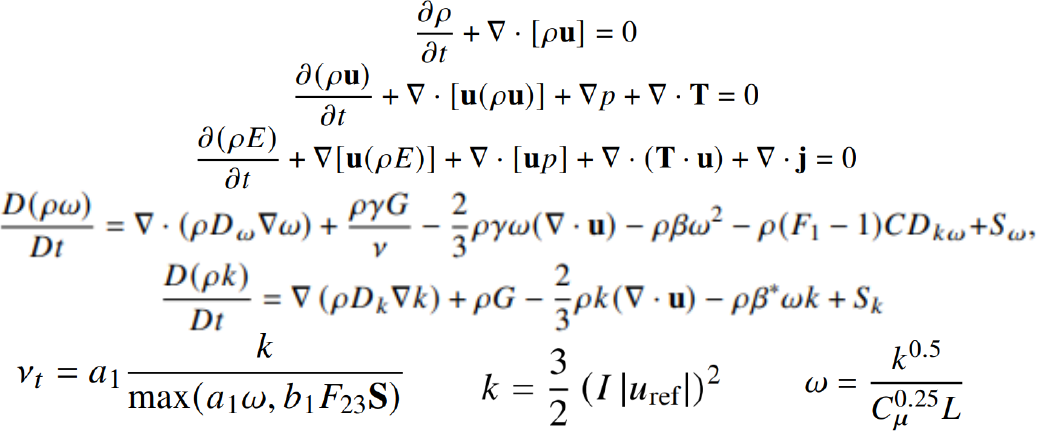
\includegraphics[width=\linewidth]{figs/of_solver.png}
    \caption{OpenFOAM numerical solver.}
    \label{fig:OF}
\end{figure}

\begin{table}[H]
\centering
\caption{Fluent solver settings.}
\label{tab:solver_settings}
\begin{tabular}{|l|c|}
\hline
\textbf{Setting} & \textbf{Value} \\ \hline
\textbf{Equations} & \\ \hline
Flow & True \\
Turbulence & True \\ \hline
\textbf{Numerics} & \\ \hline
Absolute Velocity Formulation & True \\ \hline
\textbf{Under-Relaxation Factors} & \\ \hline
Turbulent Kinetic Energy & 0.8 \\
Specific Dissipation Rate & 0.8 \\
Turbulent Viscosity & 1 \\
Solid & 1 \\ \hline
\textbf{Discretization Scheme} & \\ \hline
Flow & Second Order Upwind \\
Turbulent Kinetic Energy & Second Order Upwind \\
Specific Dissipation Rate & Second Order Upwind \\ \hline
\textbf{Time Marching} & \\ \hline
Solver & Implicit \\
Courant Number & 0.1-4 \\ \hline
\end{tabular}
\end{table}

\begin{table}[H]
\centering
\caption{Summary of relevant boundary conditions in Fluent.}
\label{tab:bc_summary}
\resizebox{\textwidth}{!}{%
\begin{tabular}{|l|c|c|c|c|}
\hline
\rowcolor[HTML]{EFEFEF} 
\textbf{Boundary Type} & \textbf{Velocity [m/s]} & \textbf{Pressure [Pa]} & \textbf{Temperature [K]} & \textbf{Turbulence (\%, Ratio)} \\ \hline

Inlet & 3.43 (Normal) & 408239 (Supersonic) & 295 & 3\%, 10 \\ \hline
Outlet & -- & 0 (Backflow) & 295 & 3\%, 10 \\ \hline
Freestream & -- & 0 (Backflow) & 295 & 3\%, 10 \\ \hline
Wall   & No Slip & -- & Adiabatic (0 Heat Flux) & -- \\ \hline
Symmetry & -- & -- & -- & -- \\ \hline
\end{tabular}%
}
\end{table}

\begin{table}[H]
\centering
\caption{Material properties.}
\label{tab:material_properties}
\resizebox{0.75\textwidth}{!}{%
\begin{tabular}{|>{\columncolor[HTML]{EFEFEF}}l|c|c|}
\hline
\rowcolor[HTML]{EFEFEF}
\textbf{Property} & \textbf{Value} \\ \hline
Density Model & Ideal Gas \\ \cline{1-2}
Specific Heat ($C_p$) & NASA 9-piecewise polynomial \\ \cline{1-2}
Thermal Conductivity & Piecewise Linear \\ \cline{1-2}
Viscosity Model & Sutherland Law \\ \cline{1-2}
Molecular Weight & 28.966 kg/kmol \\ \hline
Density & 2719 kg/m$^3$ \\ \cline{1-2}
Specific Heat ($C_p$) & 871 J/(kg$\cdot$K) \\ \cline{1-2}
Thermal Conductivity & 202.4 W/(m$\cdot$K) \\ \hline
\end{tabular}%
}
\end{table}

%%%%%%%%%%%%%%%%%%%%%%%%%%%%%%%%%%%%%%%%%%%%%%%%%%%
\section{Grid convergence}\label{sec:conv}
%%%%%%%%%%%%%%%%%%%%%%%%%%%%%%%%%%%%%%%%%%%%%%%%%%%
Three different grid resolutions were used: \uline{\textbf{coarse} with 244728 grid points}, \textbf{medium} with 353073 grid points, and \textbf{fine} with 418218 grid points to ensure the spatial convergence. Grid details are summarized in Table~\ref{tab:convergence_study}.

Figure~\ref{fig:convS} and~\ref{fig:convT}, respectively shows the spatial and temporal evolution of the temperature field on the three grid levels. It can be seen that 0.1 seconds is sufficient to achieve a time-convergent solution for this case.

\begin{table}[H]
\centering
\caption{Grid resolutions and time convergence for temperature field simulation.}
\label{tab:convergence_study}
\begin{tabular}{ccc}
\hline
\textbf{Grid Resolution} & \textbf{Number of Grid Points} & \textbf{Time for Convergence (s)} \\ \hline
Coarse                   & 244728                      & 0.1                             \\ \hline
Medium                   & 353073                      & 0.1                             \\ \hline
Fine                     & 418218                      & 0.1                             \\ \hline
\end{tabular}
\end{table}

\begin{figure}[H]
    \centering
    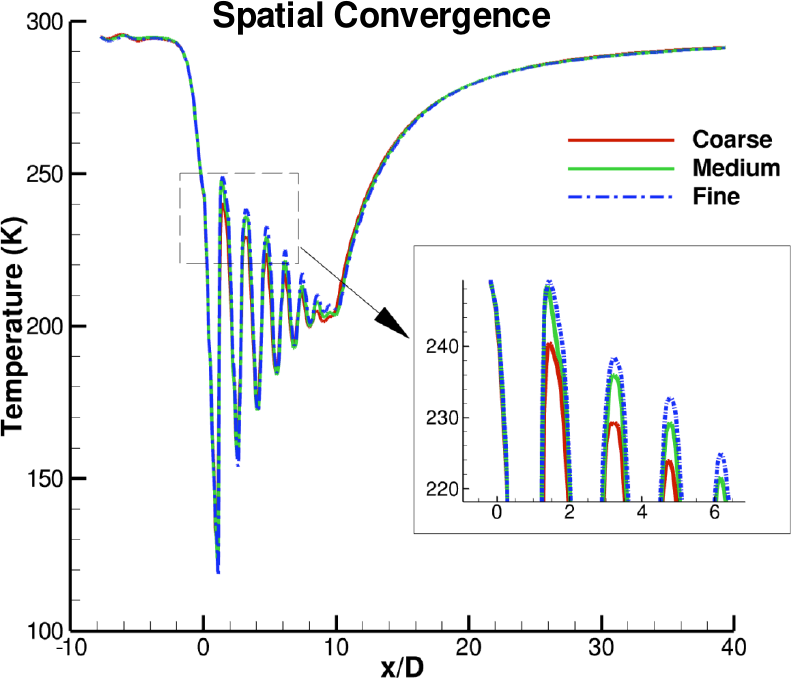
\includegraphics[width=0.7\linewidth]{figs/f3.png}\\
    %\vspace{0.5cm}
    %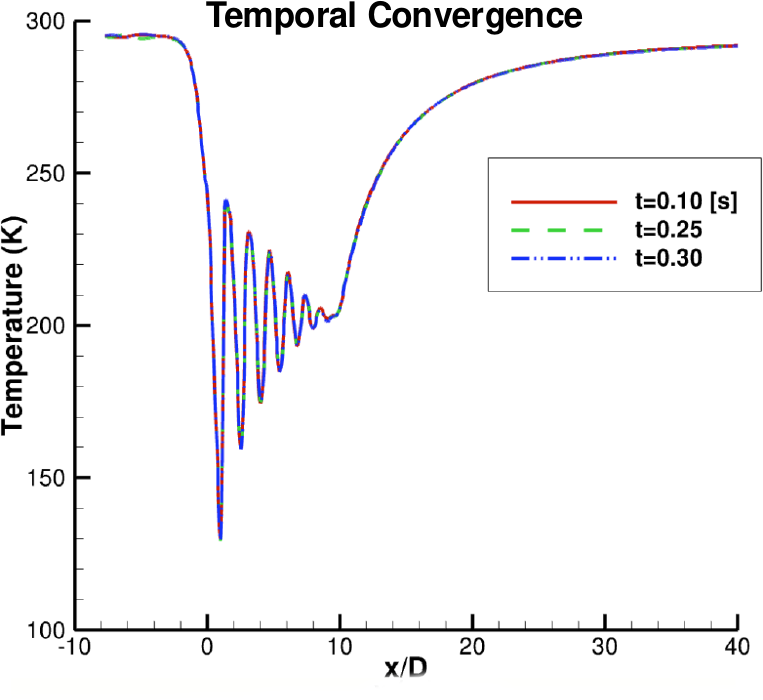
\includegraphics[width=0.7\linewidth]{figs/f4.png}
    \caption{Spatial convergence shown for the temperature field.}
    \label{fig:convS}
\end{figure}

\begin{figure}[H]
    \centering
    %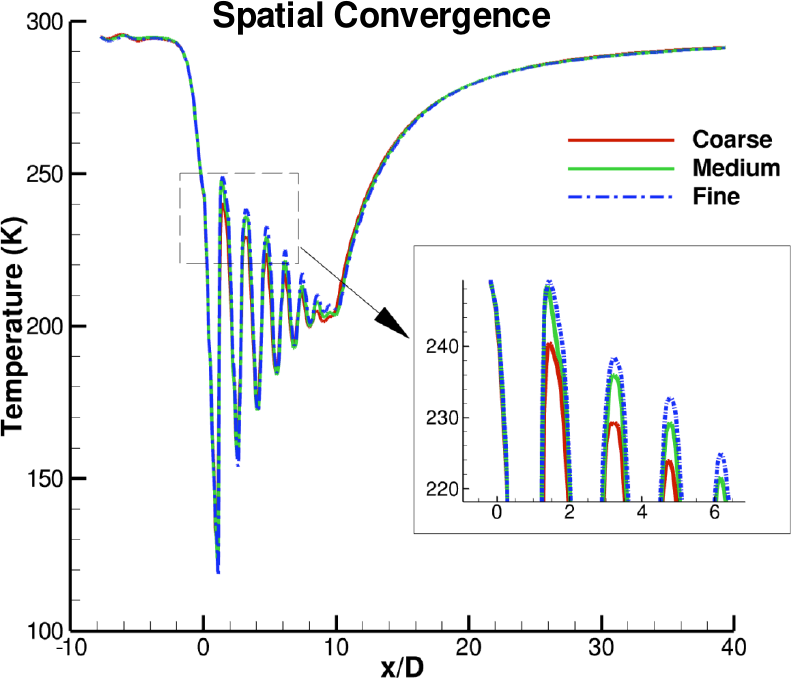
\includegraphics[width=0.7\linewidth]{figs/f3.png}\\
    %\vspace{0.5cm}
    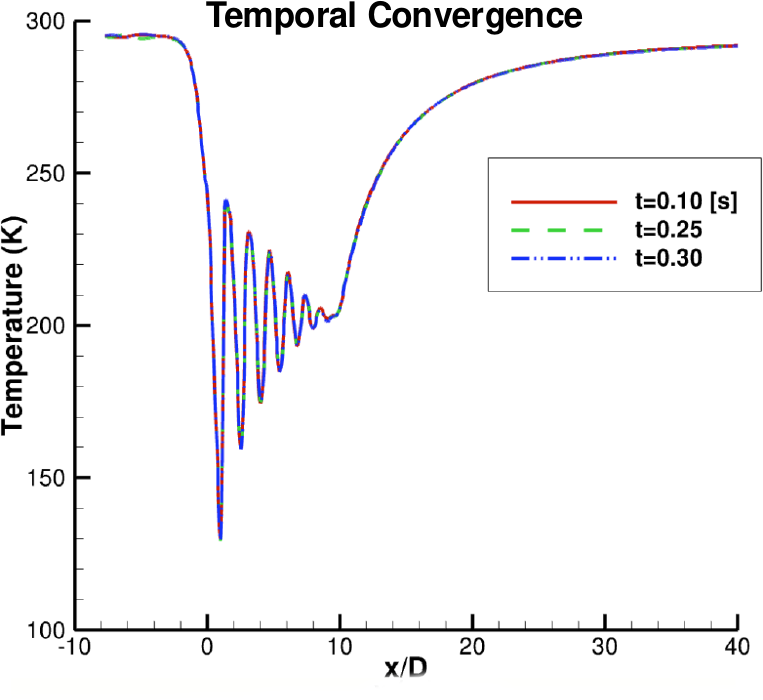
\includegraphics[width=0.7\linewidth]{figs/f4.png}
    \caption{Temporal convergence shown for the temperature field.}
    \label{fig:convT}
\end{figure}

Numerical simulation were first performed in OpenFOAM. OpenFOAM grids were then exported to Fluent mesh format using a converter utility~\cite{chitalov2021developing}. Results provided in this report were calculated on the coarse grid level.

%%%%%%%%%%%%%%%%%%%%%%%%%%%%%%%%%%%%
\section{Results}\label{sec:results}
%%%%%%%%%%%%%%%%%%%%%%%%%%%%%%%%%%%%
With the intent of validating and build trust on the results obtained by the available numerical solvers, \textbf{Fluent} and \textbf{OpenFOAM}, for the Charon (and Eris) jet-ON configuration, additional test cases have been proposed and numerically investigated in the present report. In particular, the dynamics of jet expansion across a spectrum of nozzle pressure and temperature ratios was simulated.

Results for:
\begin{itemize}
    %\item TC1: NPR=1.1, NTR=1.813
    \item TC2: NPR=4.03, NTR=1.0
\end{itemize}
%NPR=1.1, NTR=1.813 and NPR=4.03, NTR=1.0 
are presented, whose detail initial conditions (ICs) are provided in Table~\ref{tab:test_matrix}. Experimental data is available %for both, respectively, in~\cite{seiner1992effects} 
in~\cite{henderson2005experimental} as well as numerical solutions from an independent source\footnote{Private communication with Dr. Ozgur Tumuklu (tumuko@rpi.edu). Material avaialble from:~\url{https://www.havalab.org/publications/TumukluAviation2024Jetv2Final.pdf}}.

Numerical validation considered (magnitude) velocity, Mach, static temperature and pressure, and turbulent kinetic energy (TKE) fields. The numerical results obtained with Fluent and OpenFOAM were compared with other numerical solutions and available experimental data.

%\subsection{TC1: NPR=1.1, NTR=1.813}
%$%%%%%%%%%%%%%%%%%%%%%%%%%%%%%%%%%%%%
%$
%\begin{figure}[H]
%$    \centering
%$    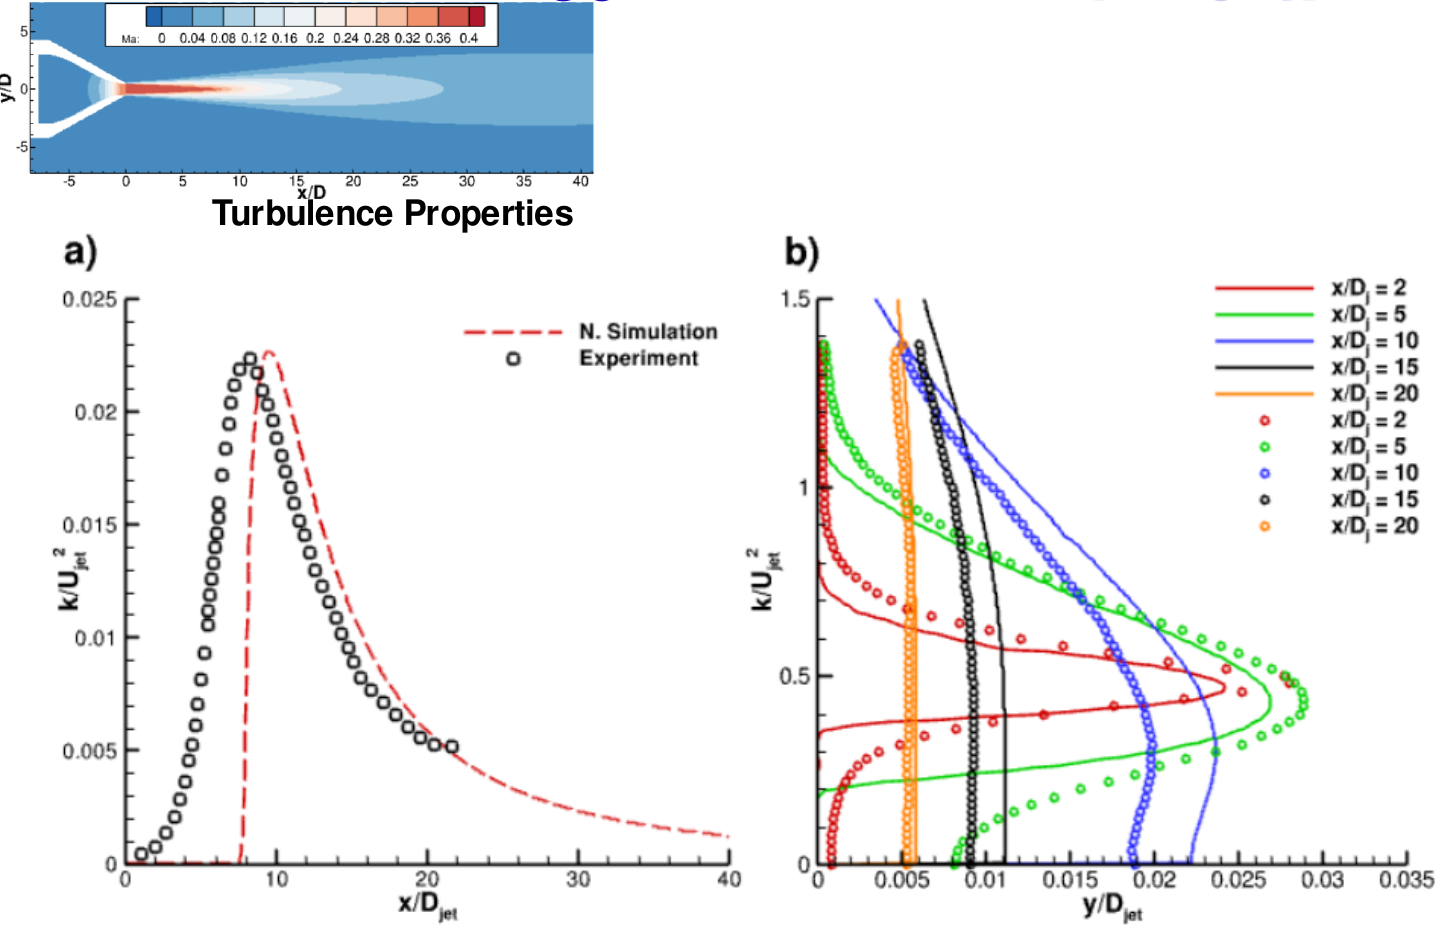
\includegraphics[width=\linewidth]{figs/f8.png}
%$    \caption{Comparisons with the \uline{experiments} from Seiner et al. (1992)~\cite{seiner1992effects}. The intensity of the TKE is maximum downstream of the core region.}
%$    \label{fig:enter-label}
%\end{figure}
%$
%\begin{figure}[H]
%$    \centering
%$    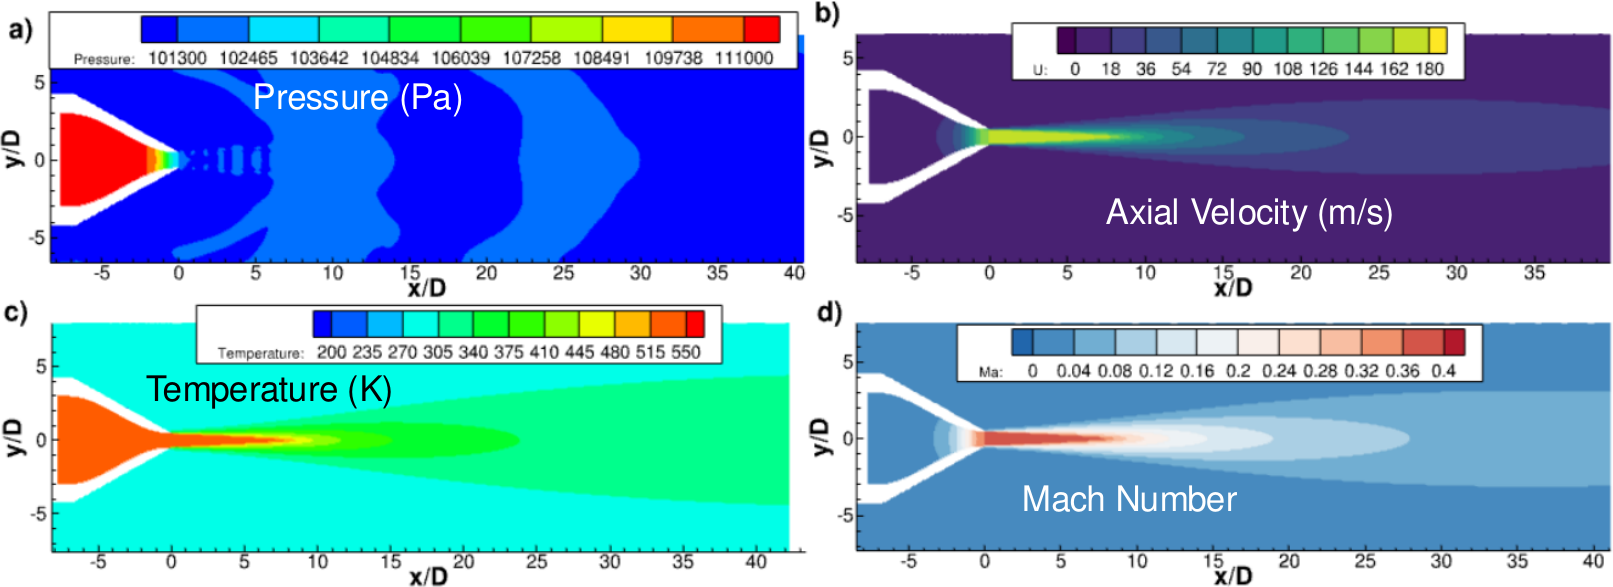
\includegraphics[width=\linewidth]{figs/f7.png}
%$    \caption{Expansion characteristics for \hl{NPR=1.1 and NTR=1.813}. Further comparisons with \uline{experiments} from Seiner et al. (1992)~\cite{seiner1992effects} were carried out to compare mean and turbulent flow properties at a low NPR.}
%$    \label{fig:enter-label}
%\end{figure}

\subsection{TC2: NPR=4.03, NTR=1}
%%%%%%%%%%%%%%%%%%%%%%%%%%%%%%%%%

\begin{figure}[H]
    \centering
    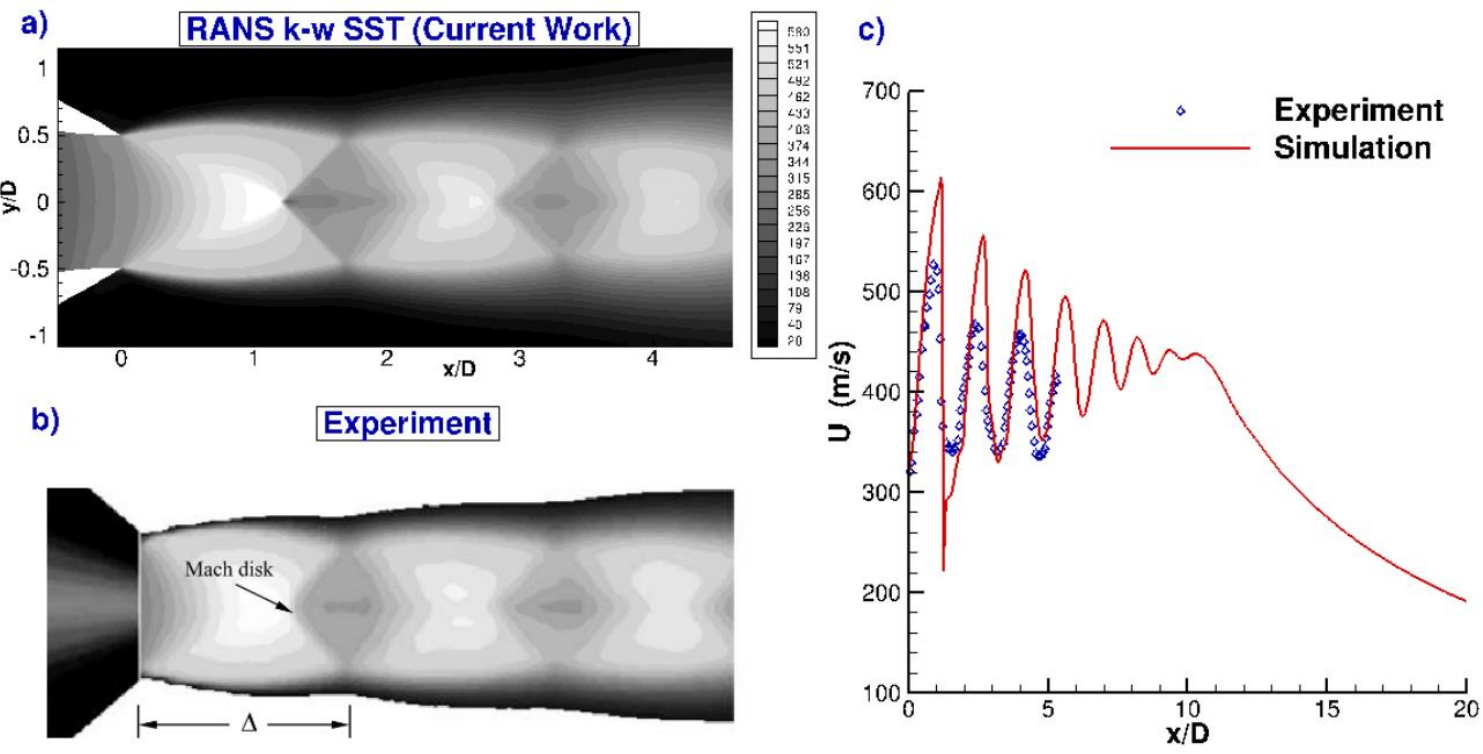
\includegraphics[width=\linewidth]{figs/f6.png}
    \caption{Comparisons with the \uline{experiments} from Henderson et al. (2005)~\cite{henderson2005experimental}. The mean velocity magnitude is in good agreement with the measurements. The differences can be attributed to the resolution limitations that cannot be captured by the cameras and the possible smearing of data during post-processing of the experiment.}
    \label{fig:enter-label}
\end{figure}

\begin{figure}[H]
    \centering
    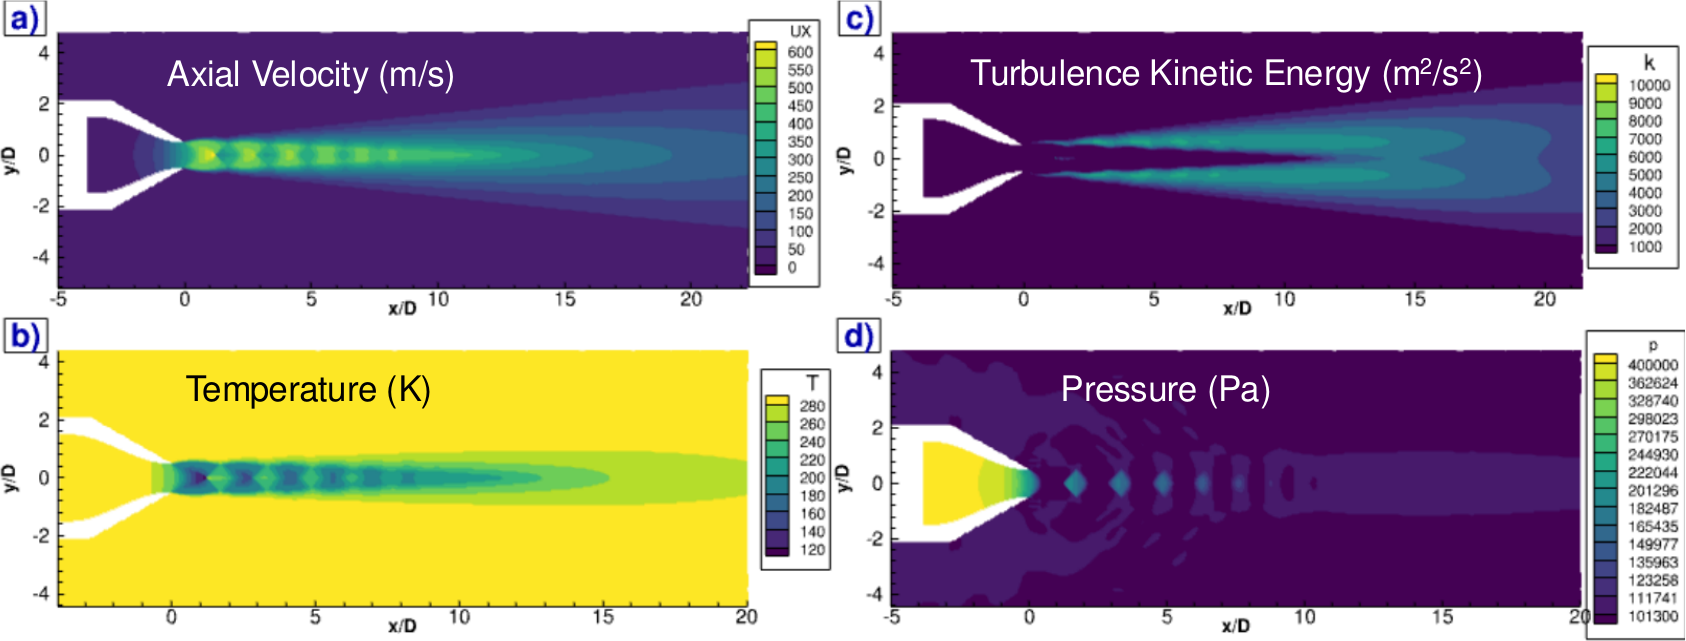
\includegraphics[width=\linewidth]{figs/f5.png}
    \caption{Expansion characteristics for \hl{NPR=4.03 and NTR=1}. The mean axial velocity peaks at approximately twice the nozzle exit velocity (317 m/s) at the jet center. The turbulence kinetic energy is maximum in the mixing layer. The propagation of the acoustic waves is seen in the pressure field. Numerical solutions provided by Dr. Ozgur Tumuklu, Assistant Professor, Aerospace Engineering, Rensselaer Polytechnic Institute, Hypersonic Aerothermal Vehicle Analysis Laboratory \url{https://www.havalab.org}.}
    \label{fig:ref_num-sols}
\end{figure}

Figure~\ref{fig:cfd-comp} shows the absolute static pressure, axial velocity, static temperature and turbulent kinetic energy production fields calculated by OpenFOAM and Fluent on the same number of contour levels. A qualitative good agreement was achieved for all fields with small but appreciable differences. Since the computational mesh is exactly the same, as well as the turbulence model, such differences are imputable to the different order of the numerical scheme adopted in the two solvers and the implementation of the boundary conditions. To be noted that different BCs were imposed in the solvers to represent the same physics due to the way in which the solvers work.

Quantitative comparison of numerical solutions is shown in Figures~\ref{fig:p}-\ref{fig:tke}. A very good agreement was obtained for the pressure fields in Figure~\ref{fig:p} while temperature, velocity Mach and turbulent kinetic energy (TKE) manifest some discrepancies. In particular, Figures~\ref{fig:vel_mag} and~\ref{fig:mach} compare numerical solutions with experimental data, for the velocity magnitude and Mach number, respectively. It can observed that Fluent tends to compute solutions in better agreement with experimental data, especially, at higher distance from the jet. This may point to the better dissipative/dispersive properties of the higher order scheme adopted in Fluent. Figure~\ref{fig:tke} reports the TKE profile along the centerline axis computed by the two solvers. It can be noted a lower peak of TKE production in Fluent, slightly shifted rightwards while showing a tail in good agreement with OpenFOAM.

\begin{figure}[H]
    \centering
    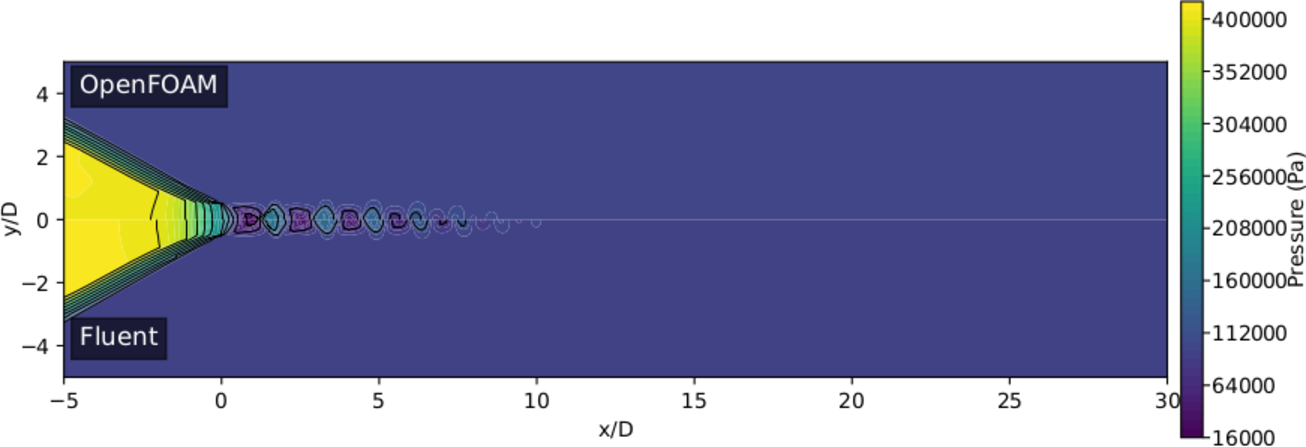
\includegraphics[width=\linewidth]{figs/P_viridis.pdf}
    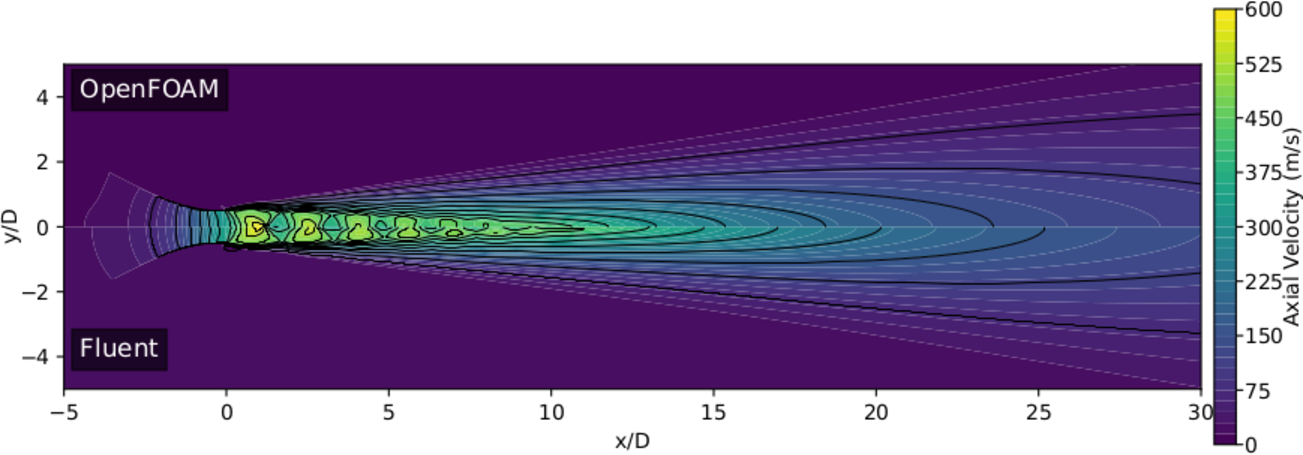
\includegraphics[width=\linewidth]{figs/U_viridis.pdf}\\
    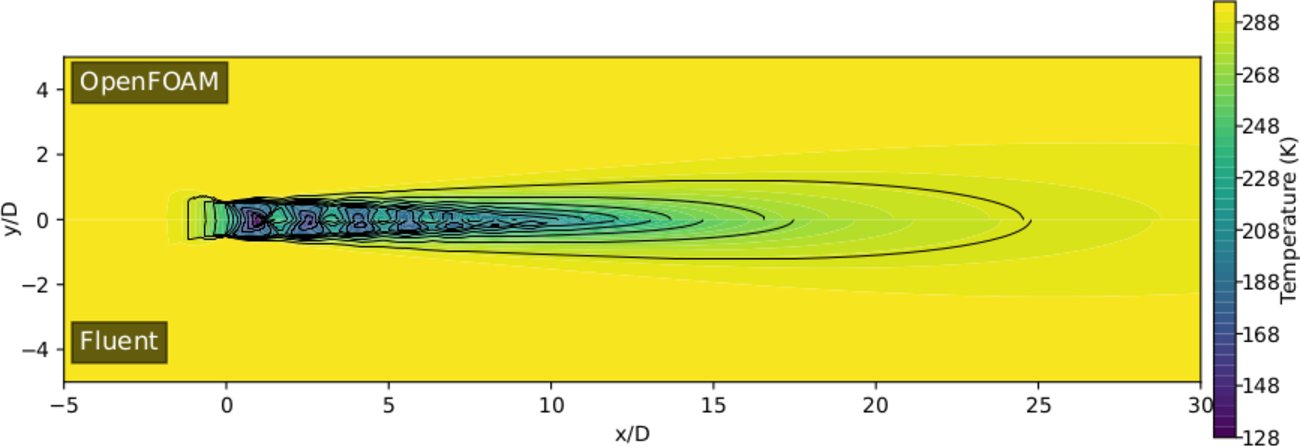
\includegraphics[width=\linewidth]{figs/T_viridis.pdf}\\
    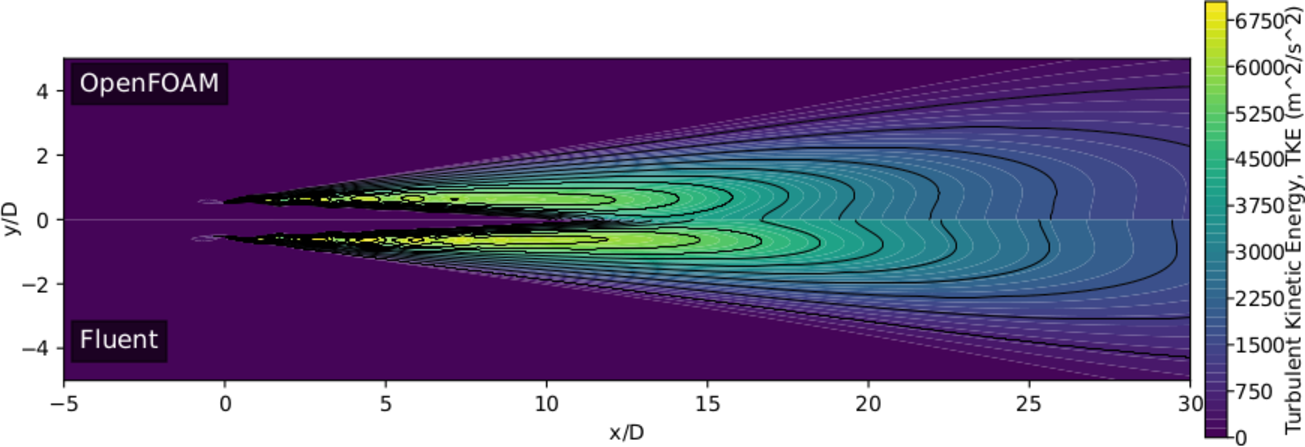
\includegraphics[width=\linewidth]{figs/TKE_viridis.pdf}\\
    %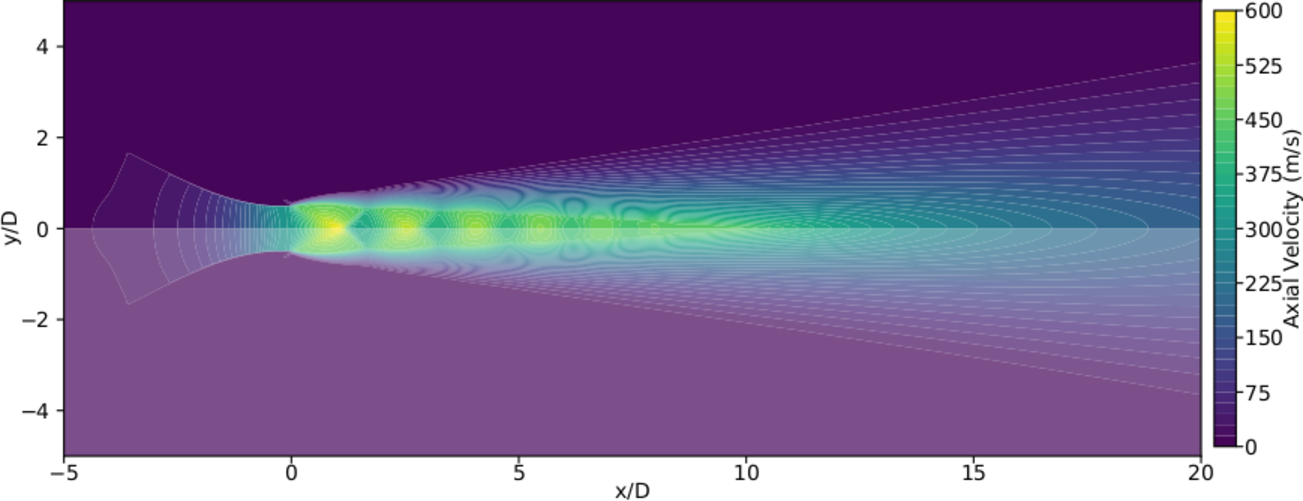
\includegraphics[width=\linewidth]{figs/rhoCentralFoam/U_viridis.pdf}\\
    %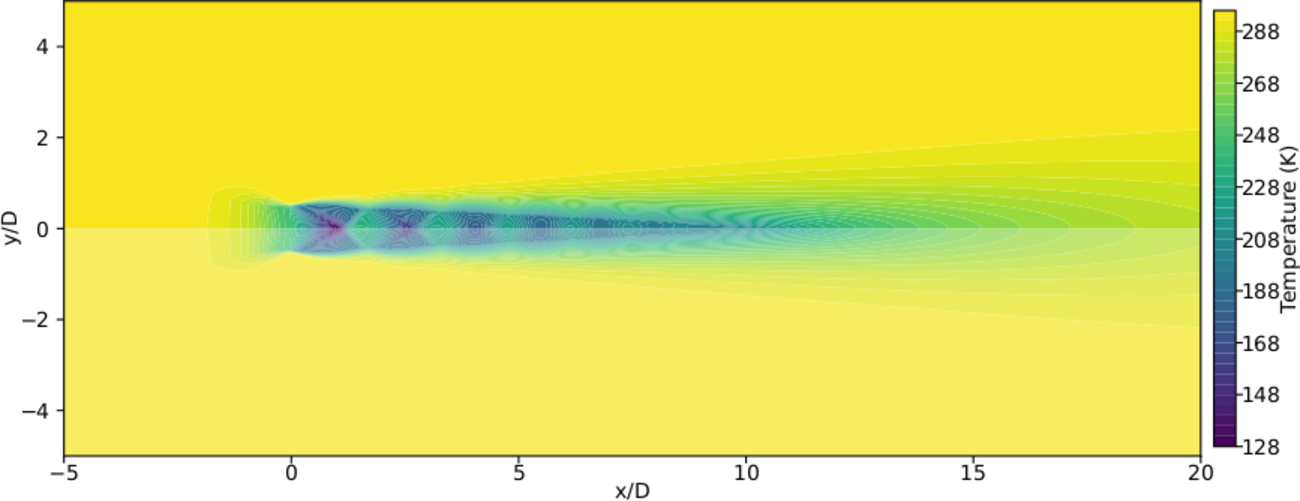
\includegraphics[width=\linewidth]{figs/rhoCentralFoam/T_viridis.pdf}\\
    %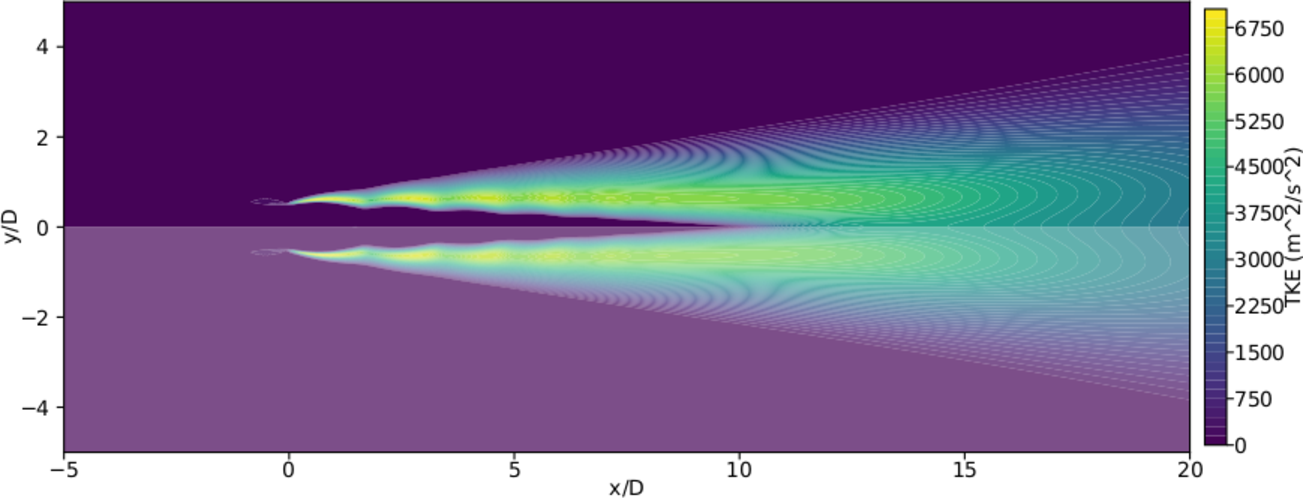
\includegraphics[width=\linewidth]{figs/rhoCentralFoam/TKE_viridis.pdf}\\
    %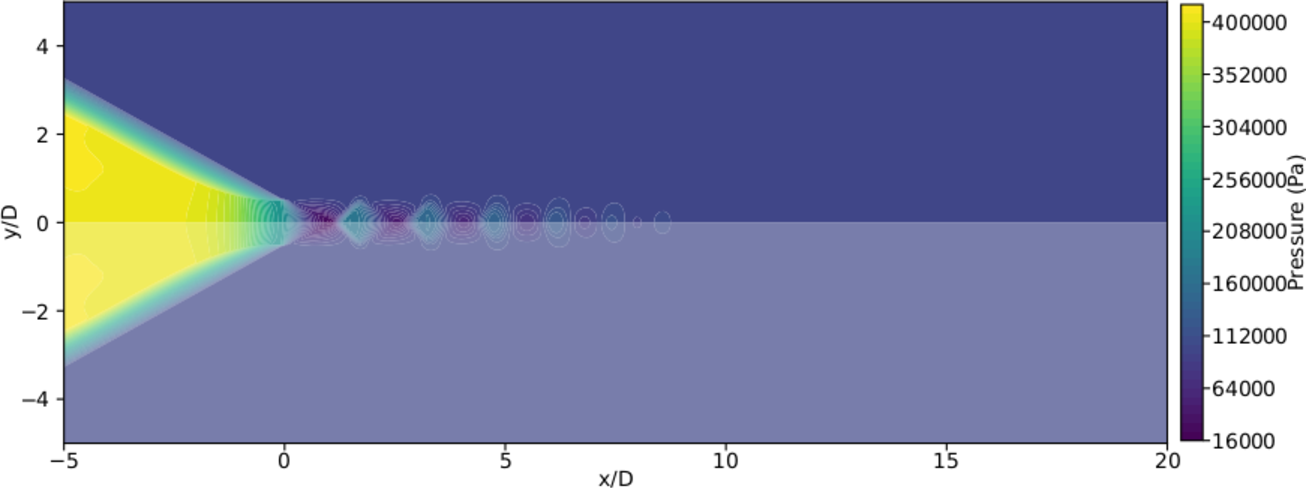
\includegraphics[width=\linewidth]{figs/rhoCentralFoam/P_viridis.pdf}
    \caption{Comparison of numerical solutions obtained by OpenFOAM and Fluent for the \hl{NPR=4.03 and NTR=1} test case. From the top: absolute pressure, axial velocity, static temperature and turbulent kinetic energy production. A constant number of levels = 11 was used for each contour.}
    \label{fig:cfd-comp}
\end{figure}

\begin{figure}[H]
    \centering
    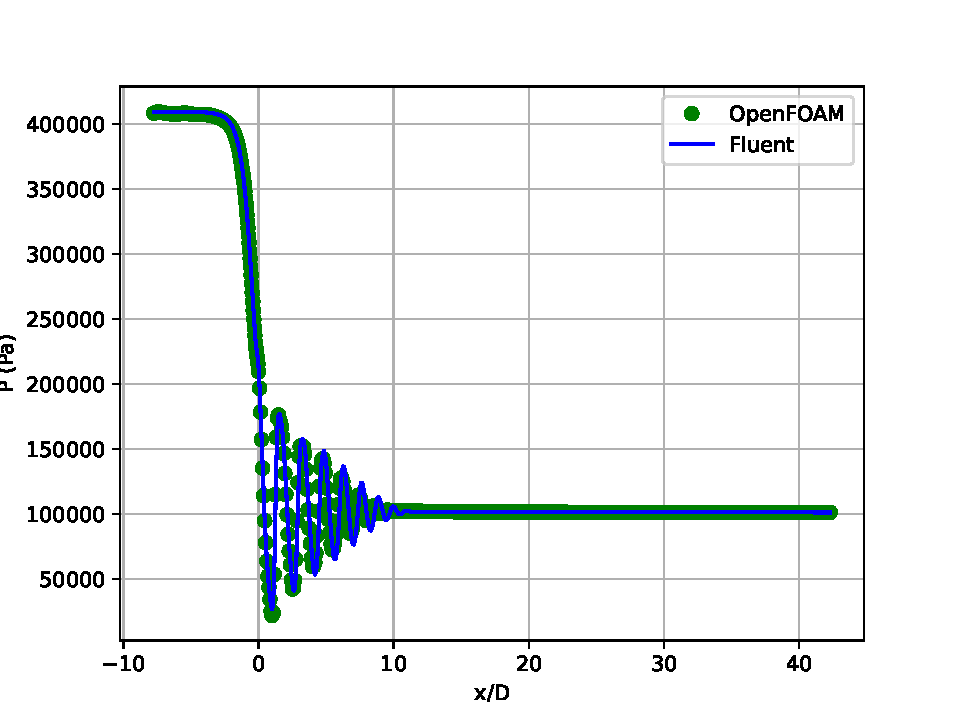
\includegraphics[width=0.925\linewidth]{figs/rhoCentralFoam/p.pdf}
    \caption{Streamwise centerline mean absolute static pressure.}
    \label{fig:p}
\end{figure}

\begin{figure}[H]
    \centering
    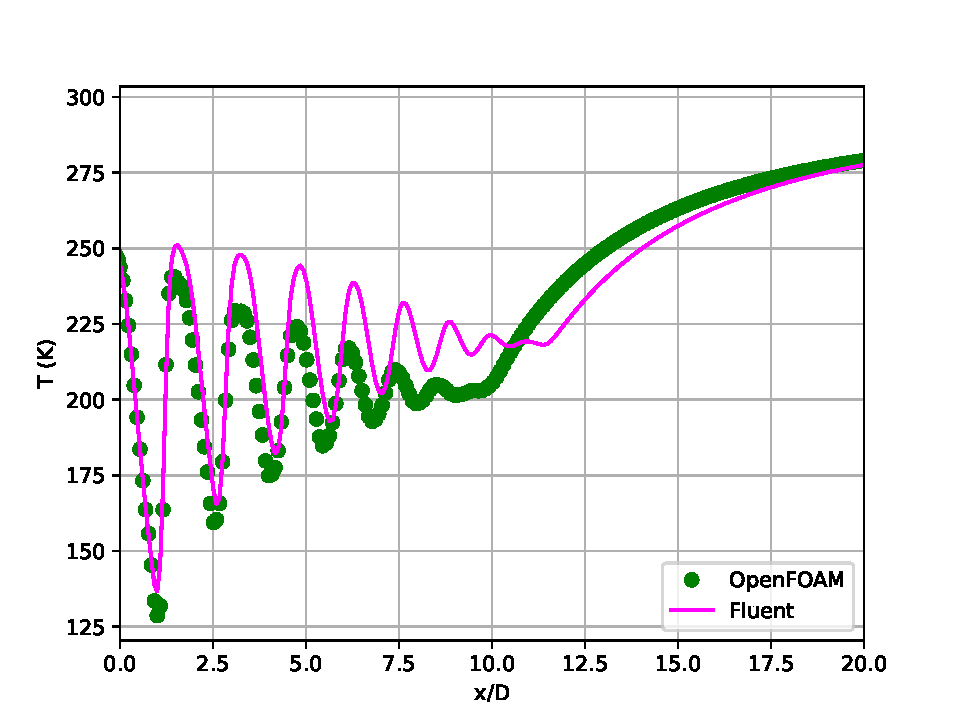
\includegraphics[width=0.925\linewidth]{figs/rhoCentralFoam/T.pdf}
    \caption{Streamwise centerline mean static temperature.}
    \label{fig:temp}
\end{figure}

\begin{figure}[H]
    \centering
    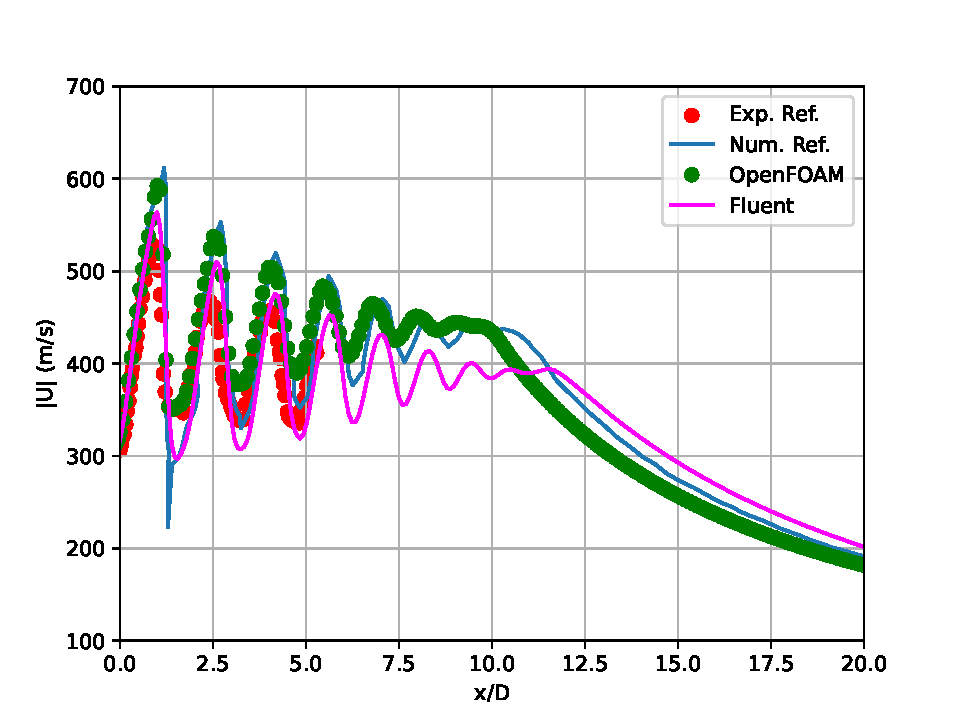
\includegraphics[width=0.925\linewidth]{figs/rhoCentralFoam/velocity_mag.pdf}
    \caption{Streamwise centerline mean velocity magnitude.}
    \label{fig:vel_mag}
\end{figure}

\begin{figure}[H]
    \centering
    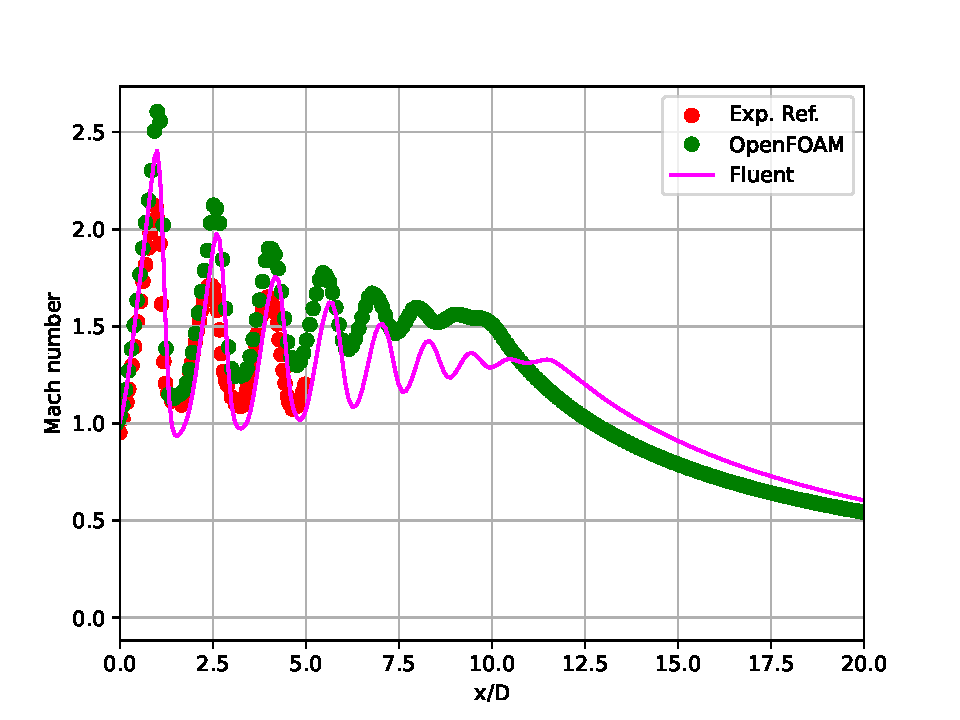
\includegraphics[width=0.925\linewidth]{figs/rhoCentralFoam/M.pdf}
    \caption{Streamwise centerline mean Mach number.}
    \label{fig:mach}
\end{figure}

\begin{figure}[H]
    \centering
    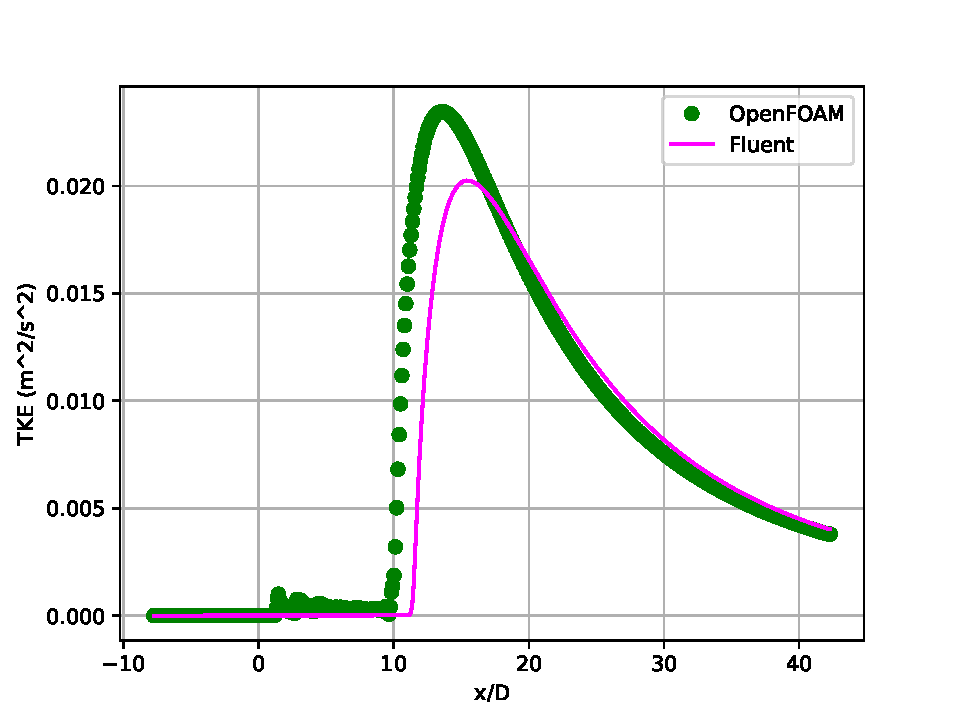
\includegraphics[width=0.925\linewidth]{figs/rhoCentralFoam/TKE.pdf}
    \caption{Streamwise centerline mean turbulent kinetic energy (TKE).}
    \label{fig:tke}
\end{figure}

%\begin{figure}[H]
%    \centering
%    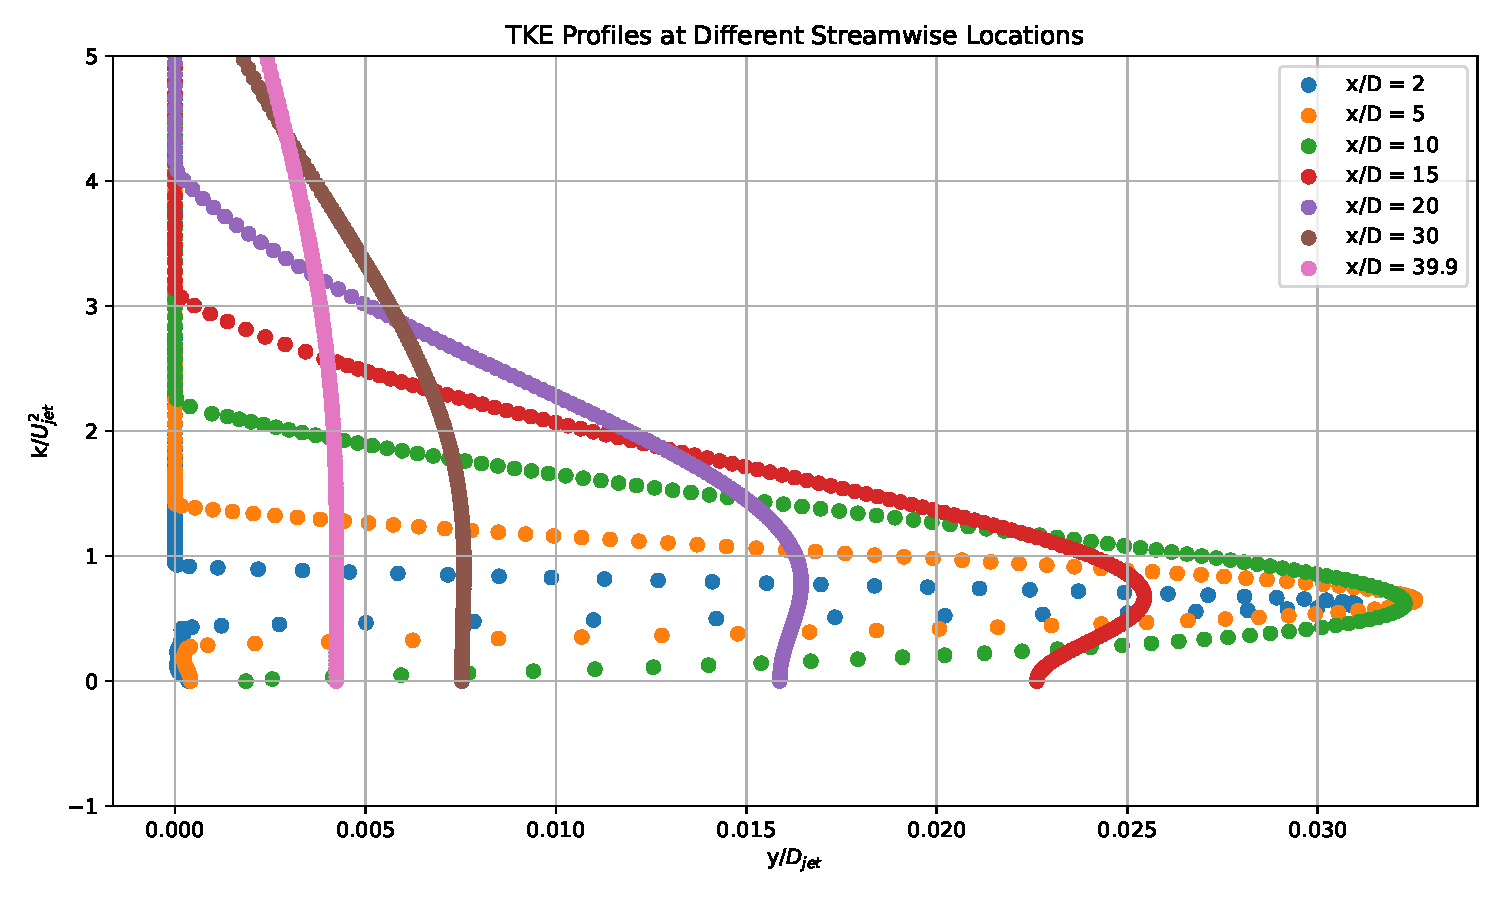
\includegraphics[width=\linewidth]{figs/rhoCentralFoam/TKE_vs_yD_at_xD_slices.pdf}
%    \caption{Streamwise centerline mean TKE.}
%    \label{fig:tke}
%\end{figure}

%\begin{figure}[H]
%    \centering
%    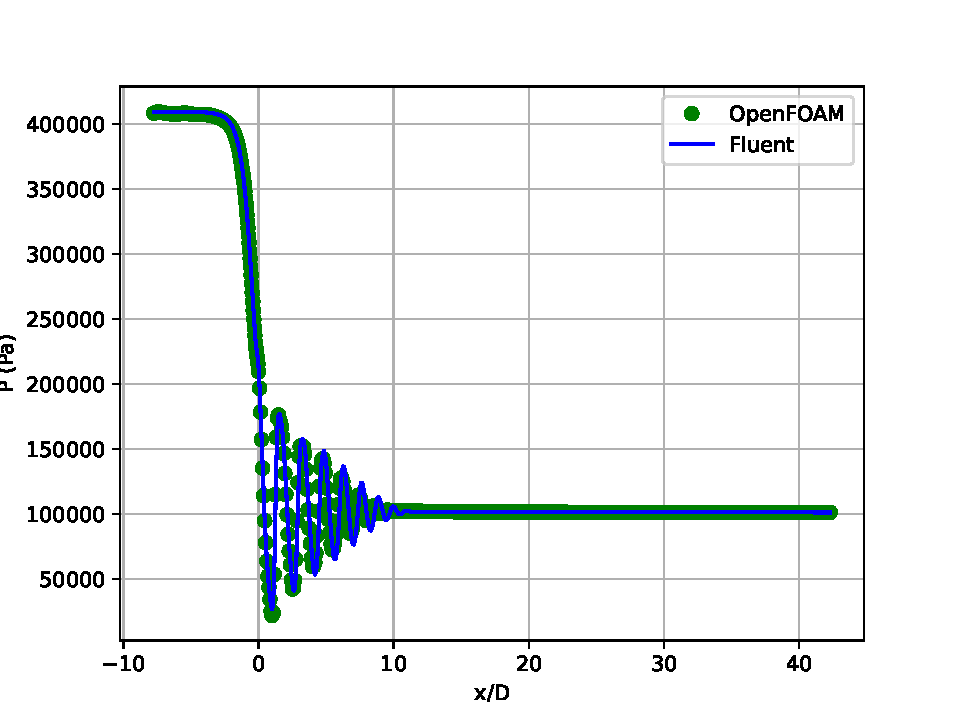
\includegraphics[width=0.495\linewidth]{figs/rhoCentralFoam/p.pdf}
%    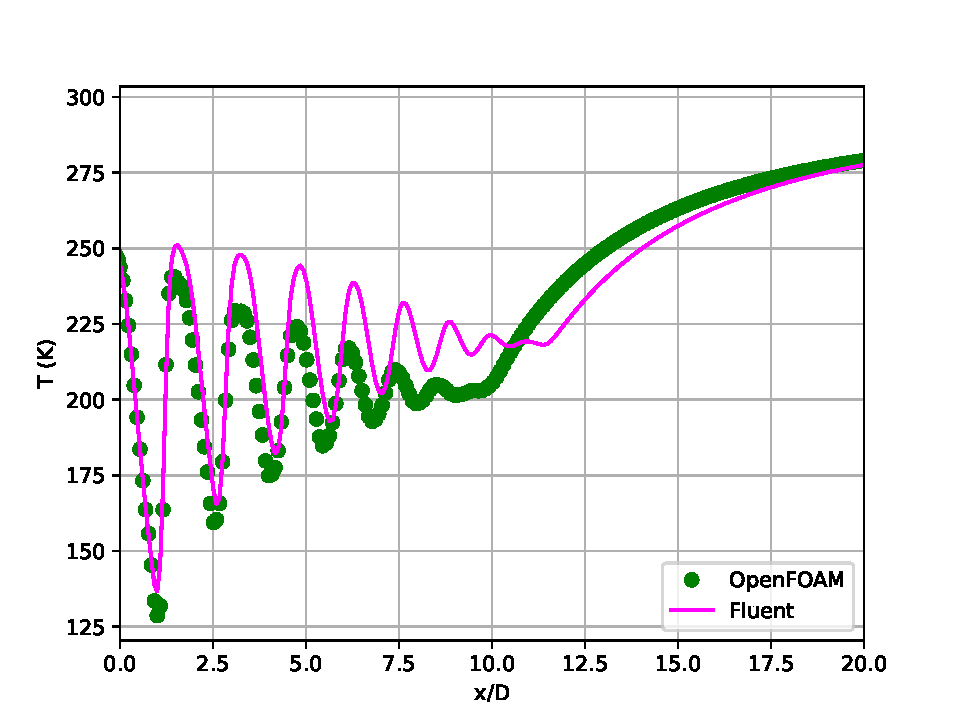
\includegraphics[width=0.495\linewidth]{figs/rhoCentralFoam/T.pdf}\\
%    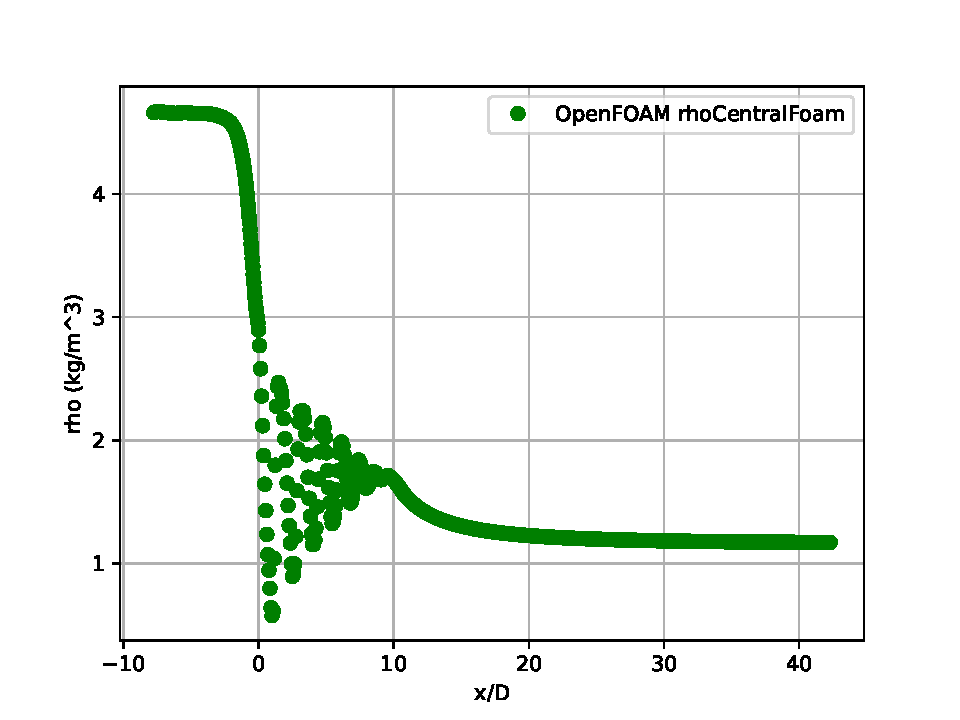
\includegraphics[width=0.495\linewidth]{figs/rhoCentralFoam/rho.pdf}
%    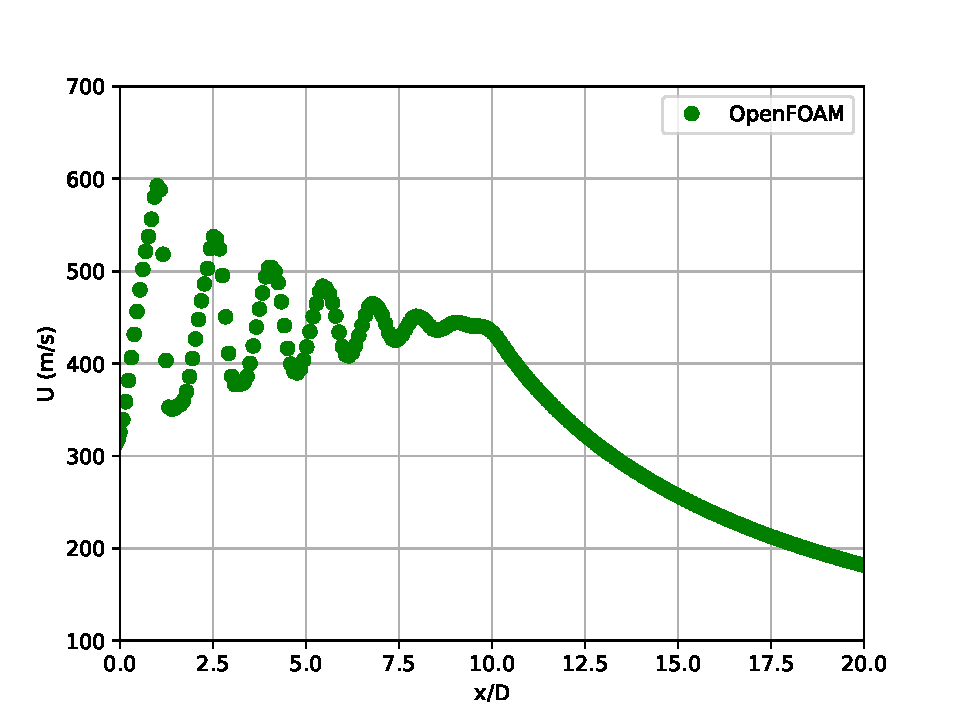
\includegraphics[width=0.495\linewidth]{figs/rhoCentralFoam/U.pdf}\\
%    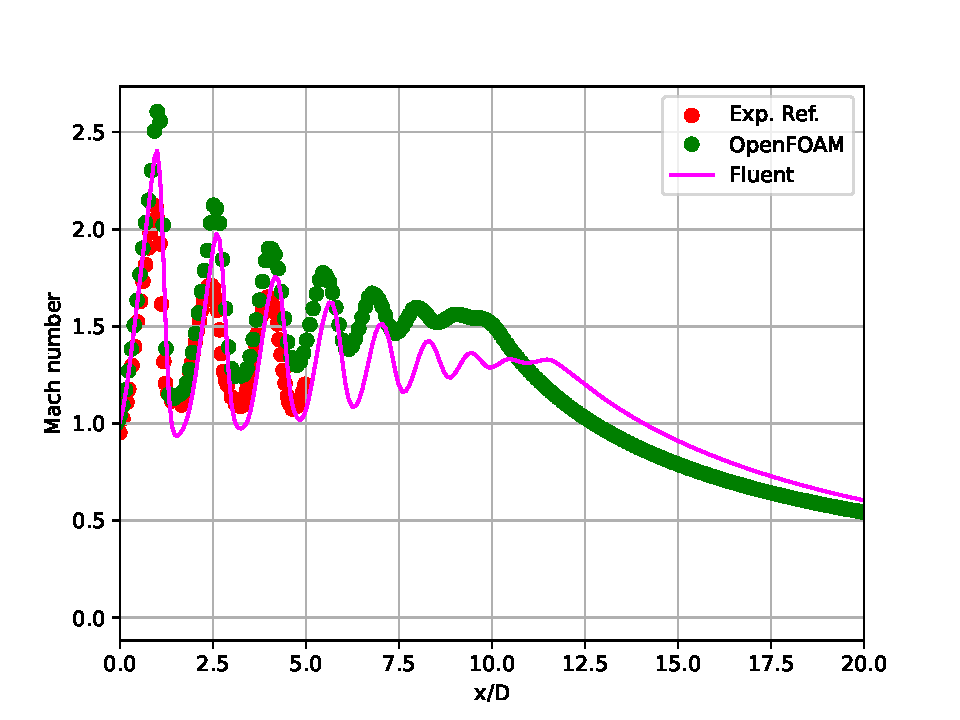
\includegraphics[width=0.495\linewidth]{figs/rhoCentralFoam/M.pdf}
%    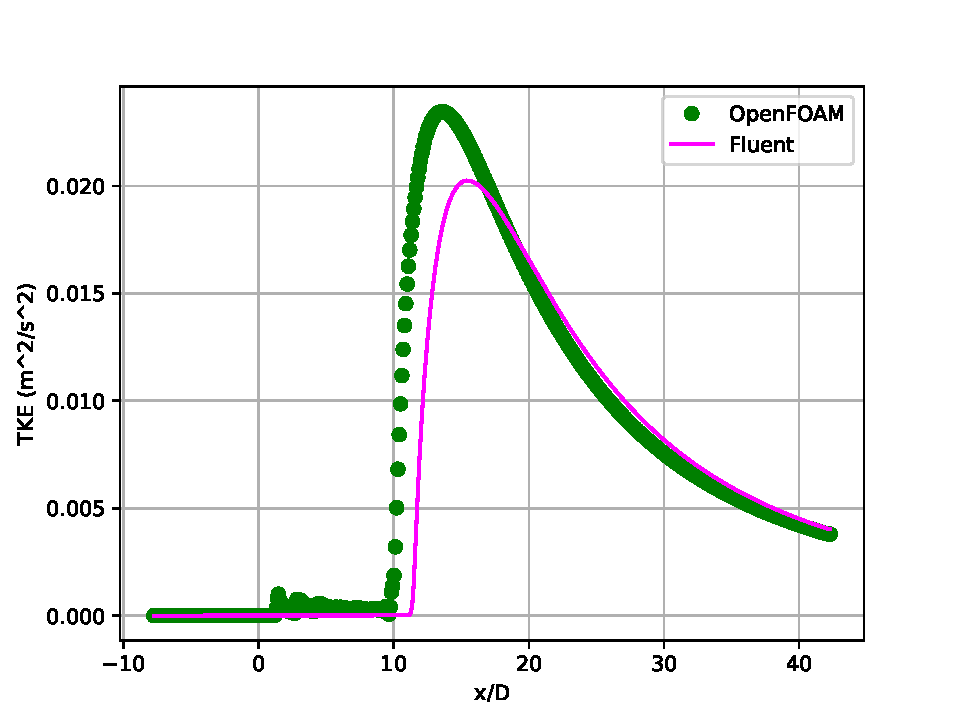
\includegraphics[width=0.495\linewidth]{figs/rhoCentralFoam/TKE.pdf}
%    \caption{Experimental and numerical streamwise centerline mean field variables.}
%    \label{fig:profile_fields}
%\end{figure}

%\subsection{TC3: NPR=4.03, NTR=8}
%%%%%%%%%%%%%%%%%%%%%%%%%%%%%%%%%%
%
%\begin{figure}[H]
%    \centering
%    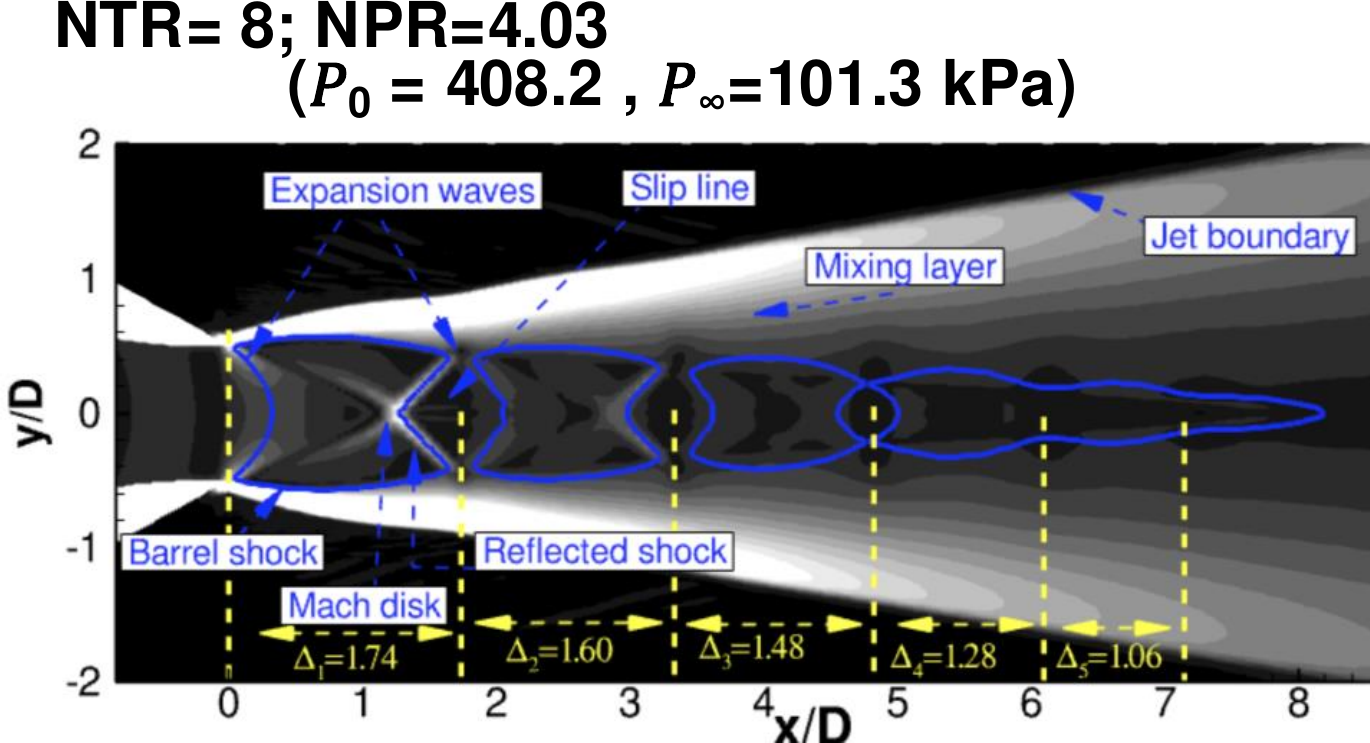
\includegraphics[width=0.95\linewidth]{figs/f1.png}\\
%    \caption{Flow-field phenomenology description for the two test cases: NPR=4.03, NTR=8.}
%    \label{fig:enter-label}
%\end{figure}
%
%\subsection{TC4: NPR=256, NTR=8}
%%%%%%%%%%%%%%%%%%%%%%%%%%%%%%%%%
%
%\begin{figure}[H]
%    \centering
%    %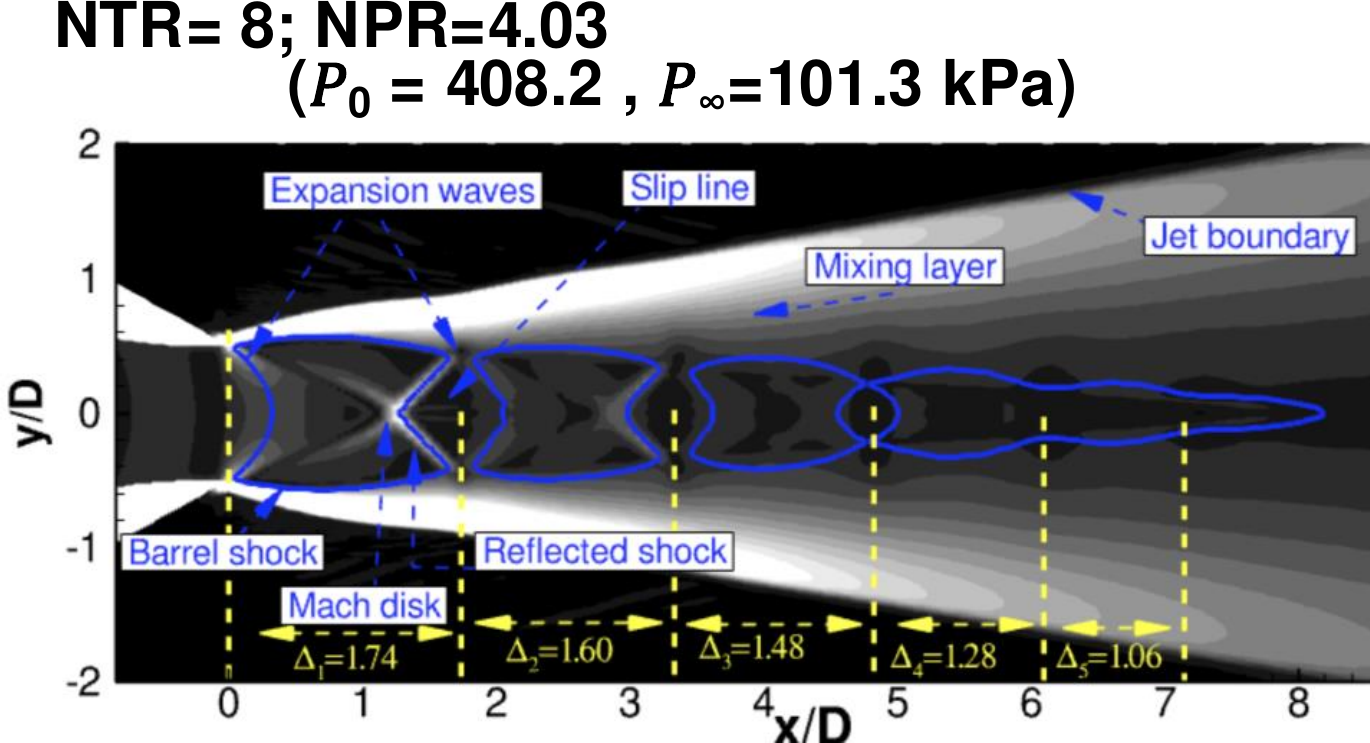
\includegraphics[width=0.95\linewidth]{figs/f1.png}\\
%    %\vspace{0.5cm}
%    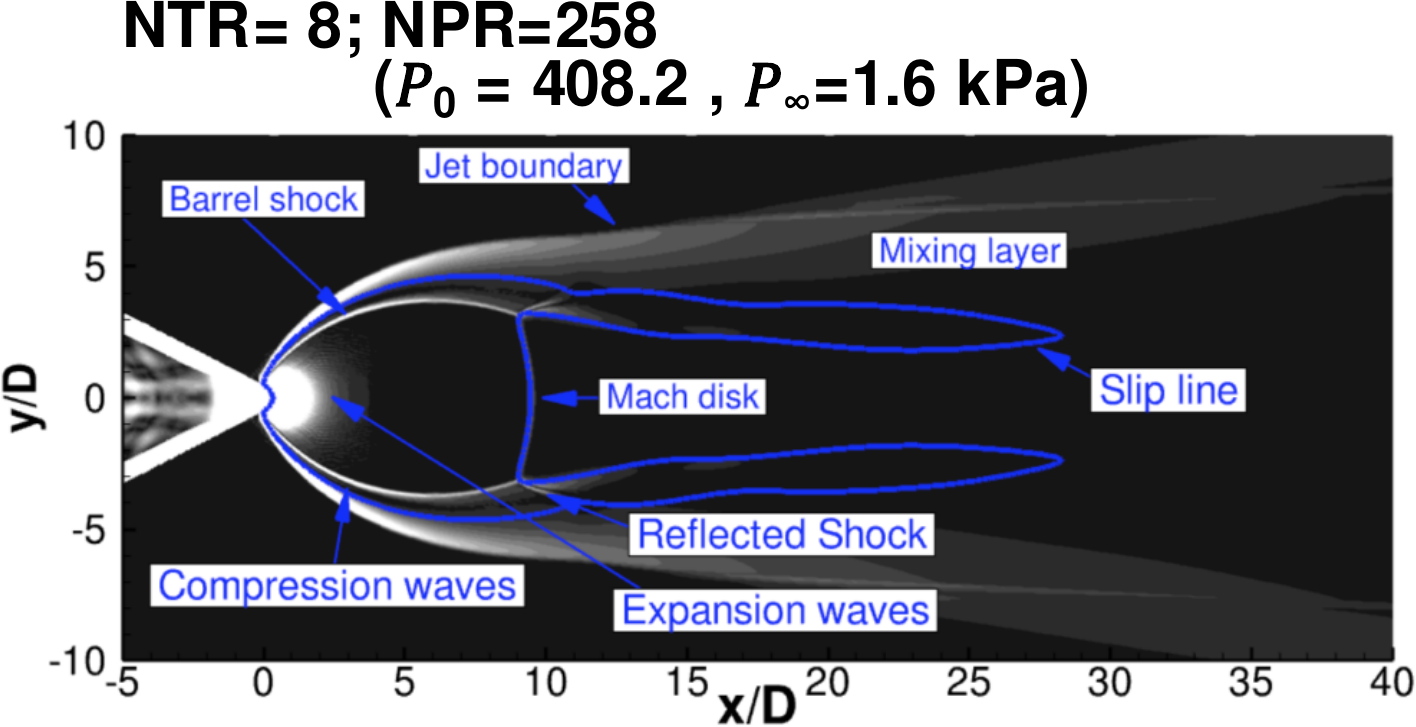
\includegraphics[width=0.95\linewidth]{figs/f2.png} 
%    \caption{Flow-field phenomenology description for the two test cases: NPR=258, NTR=8.}
%    \label{fig:enter-label}
%\end{figure}
%
%\begin{figure}[H]
%    \centering
%    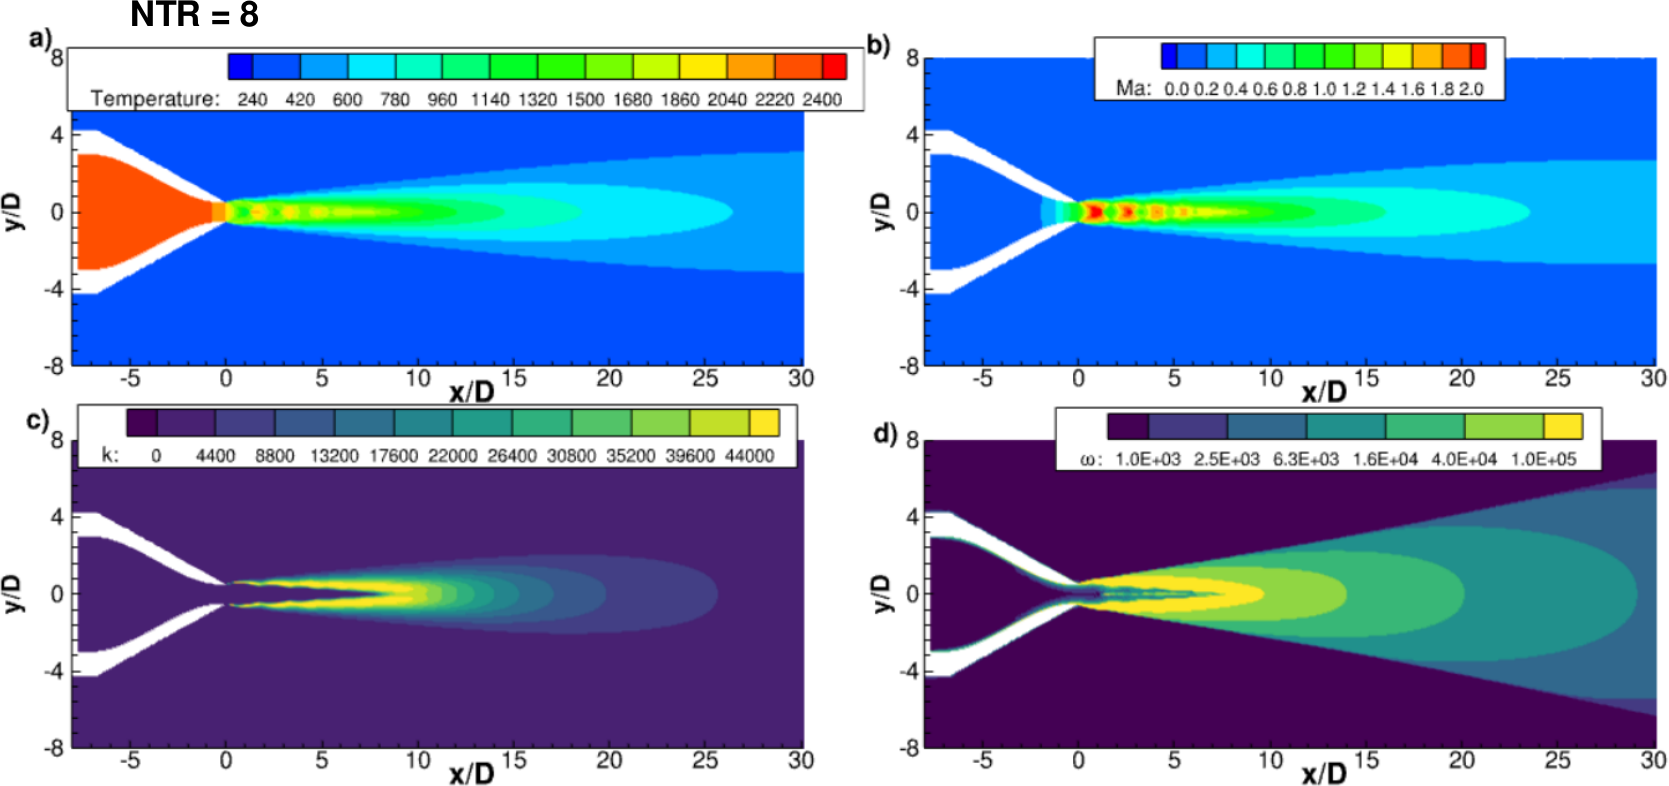
\includegraphics[width=\linewidth]{figs/f9.png}
%    \caption{Effects of NTRs on the jets for \hl{NPR=4.03}. NTR has small effect on the structure of shock diamonds. It significantly affects the turbulence properties. The number of shock diamonds decreases with higher NTRs.}
%    \label{fig:enter-label}
%\end{figure}
%
%\begin{figure}[H]
%    \centering
%    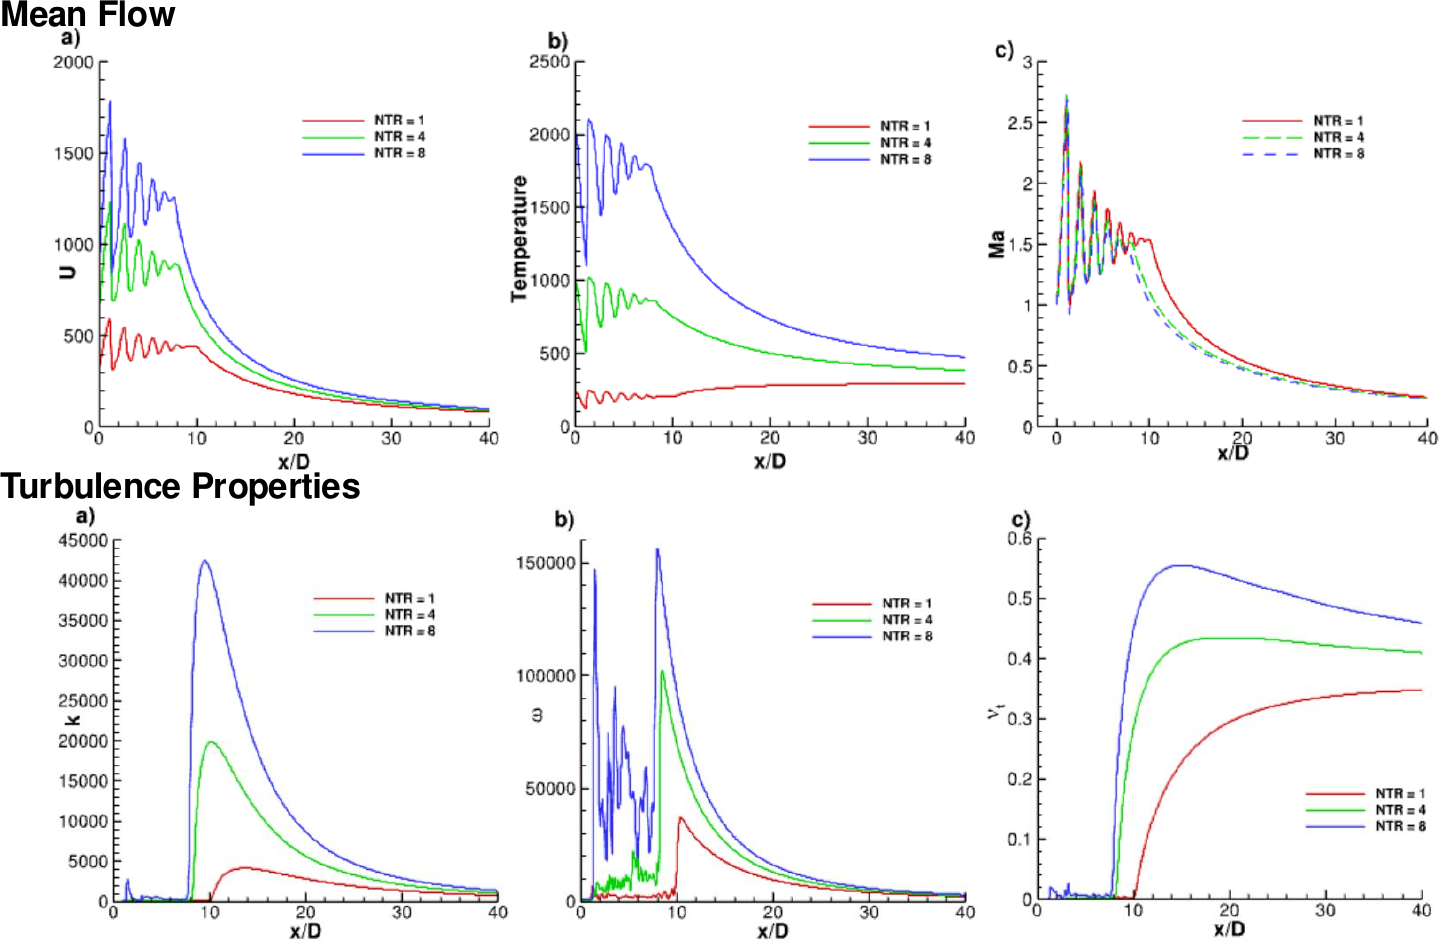
\includegraphics[width=\linewidth]{figs/f10.png}
%    \caption{Effects of NTRs on the flows~\cite{mcguirk2021near}. The turbulence kinetic energy increases almost linearly with NTR in the mixing layer.}
%    \label{fig:conv}
%\end{figure}
%
%\begin{figure}[H]
%    \centering
%    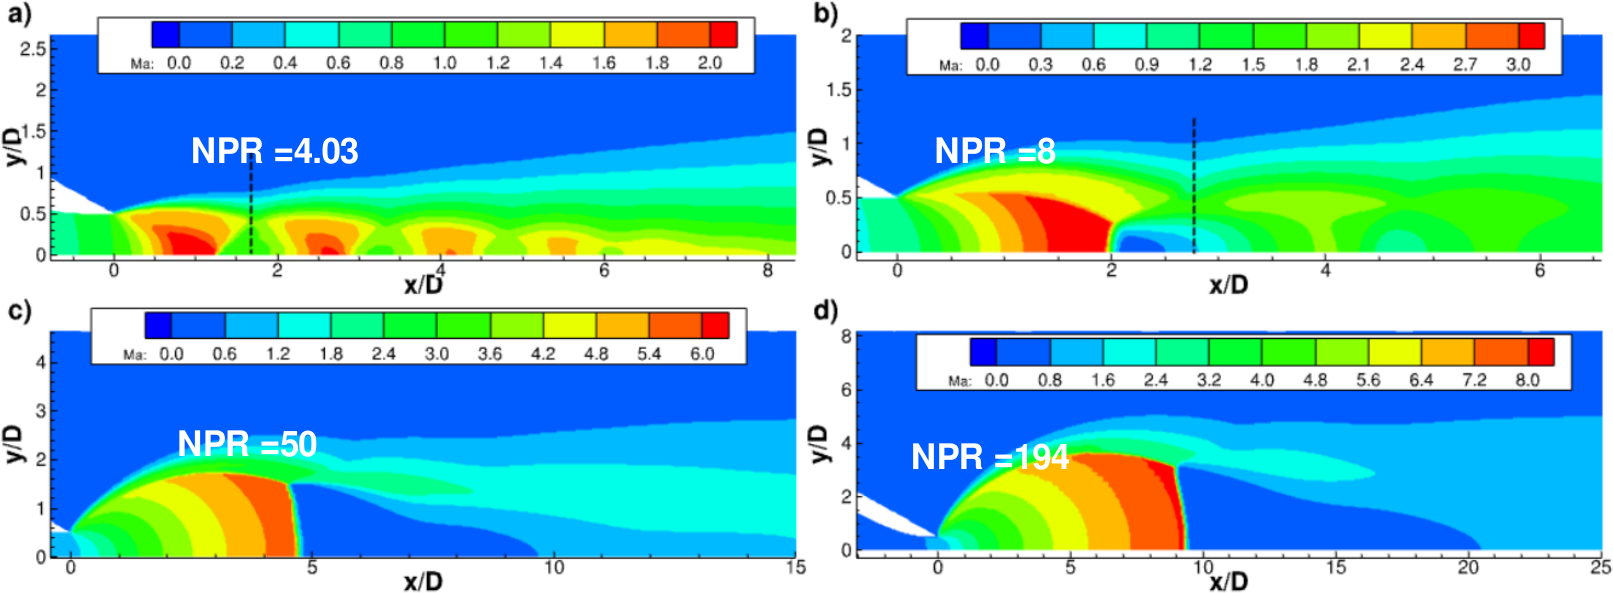
\includegraphics[width=\linewidth]{figs/f11.png}
%    \caption{Expansion characteristics for NPRs~\cite{franquet2015free}. The repetitive shock diamonds disappear with higher NPRs. The length of the first shock cell increases with NPR. The size of the Mach disk increases with NPR, and the normal shock becomes more curved.}
%    \label{fig:enter-label}
%\end{figure}
%
%\begin{figure}[H]
%    \centering
%    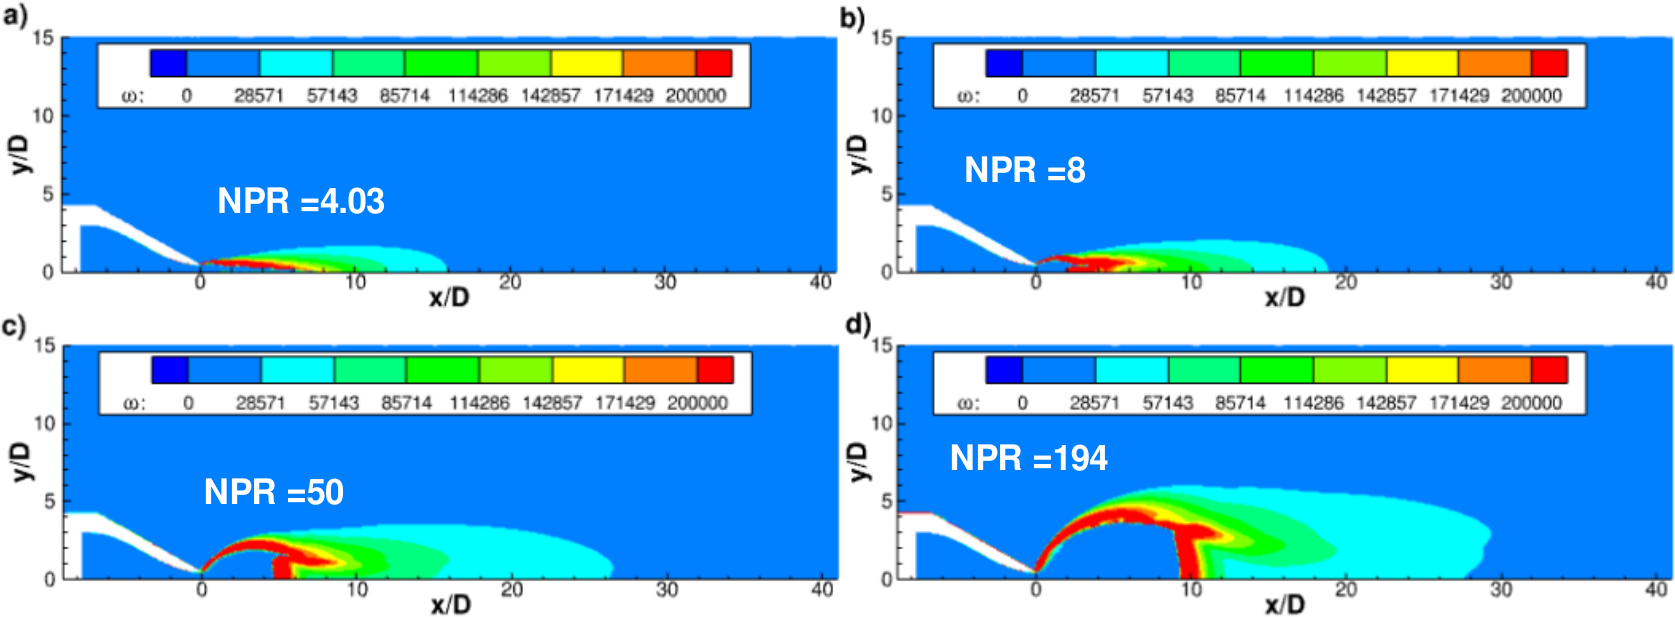
\includegraphics[width=\linewidth]{figs/f12.png}
%    \caption{Variation of turbulence parameters with NPRs. The turbulence kinetic energy significantly increases with NPR, especially in the mixing layer and downstream of the Mach disk. The size of the eddies becomes smaller downstream of the Mach disk and in the mixing layer, as indicated by the increase in specific dissipation rates at these locations.}
%    \label{fig:enter-label}
%\end{figure}
%
%\begin{figure}[H]
%    \centering
%    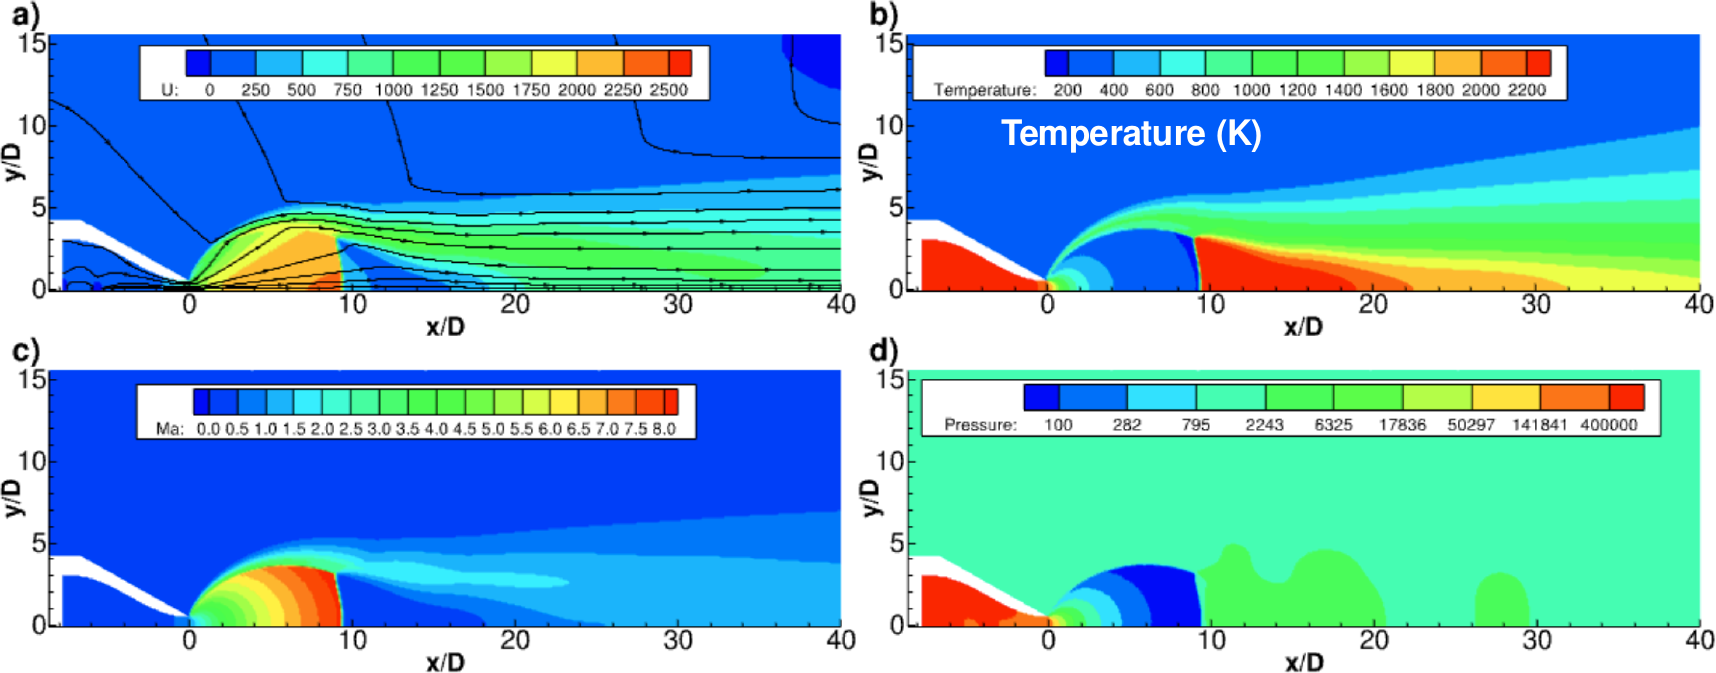
\includegraphics[width=0.95\linewidth]{figs/f13.png}
%    \caption{Flow field with \hl{NPR=256}. The streamwise velocity increases dramatically inside the potential core, while the temperature decreases to about 200 K from the stagnation temperature of 2360 K. The flow becomes hypersonic and nonequilibrium effects have to be taken into account for accurate results.}
%    \label{fig:enter-label}
%\end{figure}
%
%\begin{figure}[H]
%    \centering
%    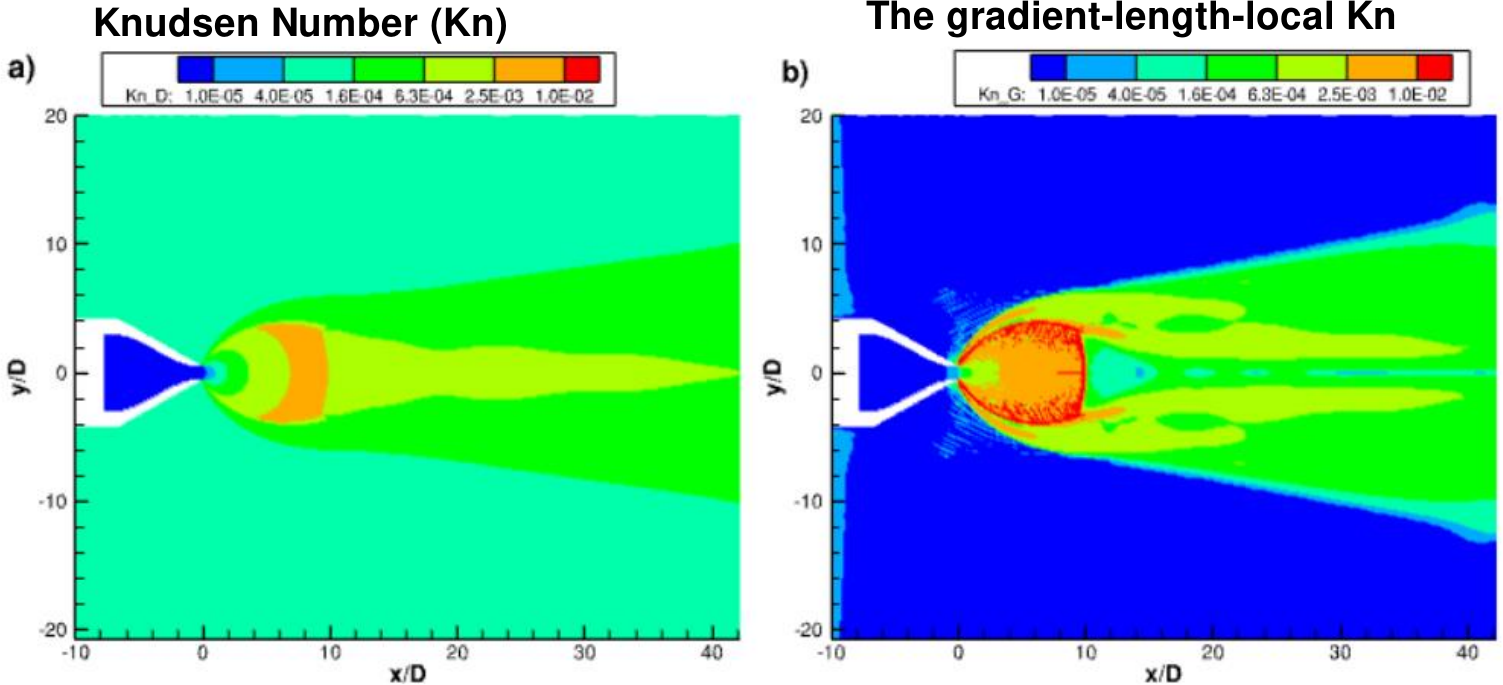
\includegraphics[width=\linewidth]{figs/f14.png}
%    \caption{Rarefied effects for \hl{NPR=256.} The nozzle-diameter-based Knudsen number, $\lambda$/D, is less than 0.01; therefore, the flow can be assumed to be in the continuum regime. On the other hand, the gradient-local-length Knudsen number becomes relatively larger, especially near the barrel shock and Mach disk.}
%    \label{fig:enter-label}
%\end{figure}
%
%\begin{figure}[H]
%    \centering
%    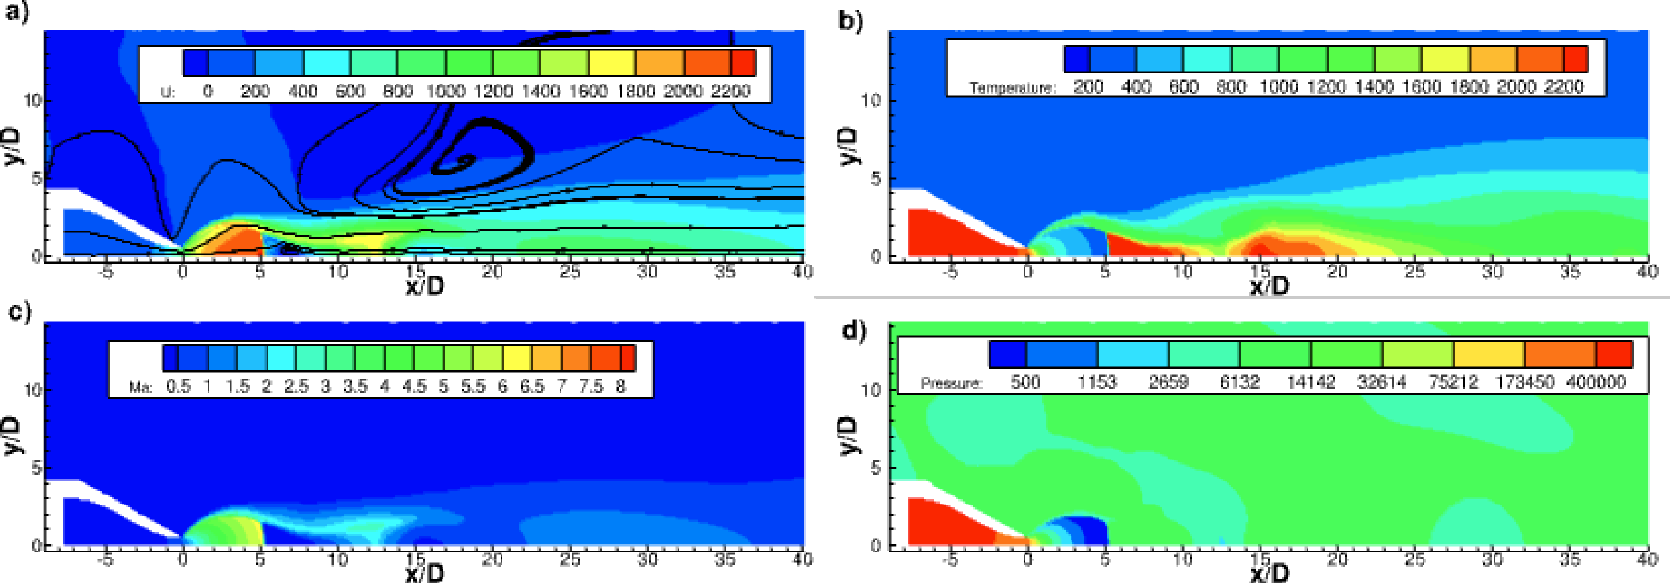
\includegraphics[width=\linewidth]{figs/f15.png}
%    \caption{Expansion characteristics for \hl{NPR=68}. The constant pressure boundary condition stipulates that the ambient pressure remains the same over time, whereas the zero-pressure gradient boundary condition allows for an increase in the pressure field since the nozzle exit pressure is higher than the ambient pressure. Oscillatory behavior is observed for the constant pressure BC when the NPR is large.}
%    \label{fig:enter-label}
%\end{figure}
%
%\begin{figure}[H]
%    \centering
%    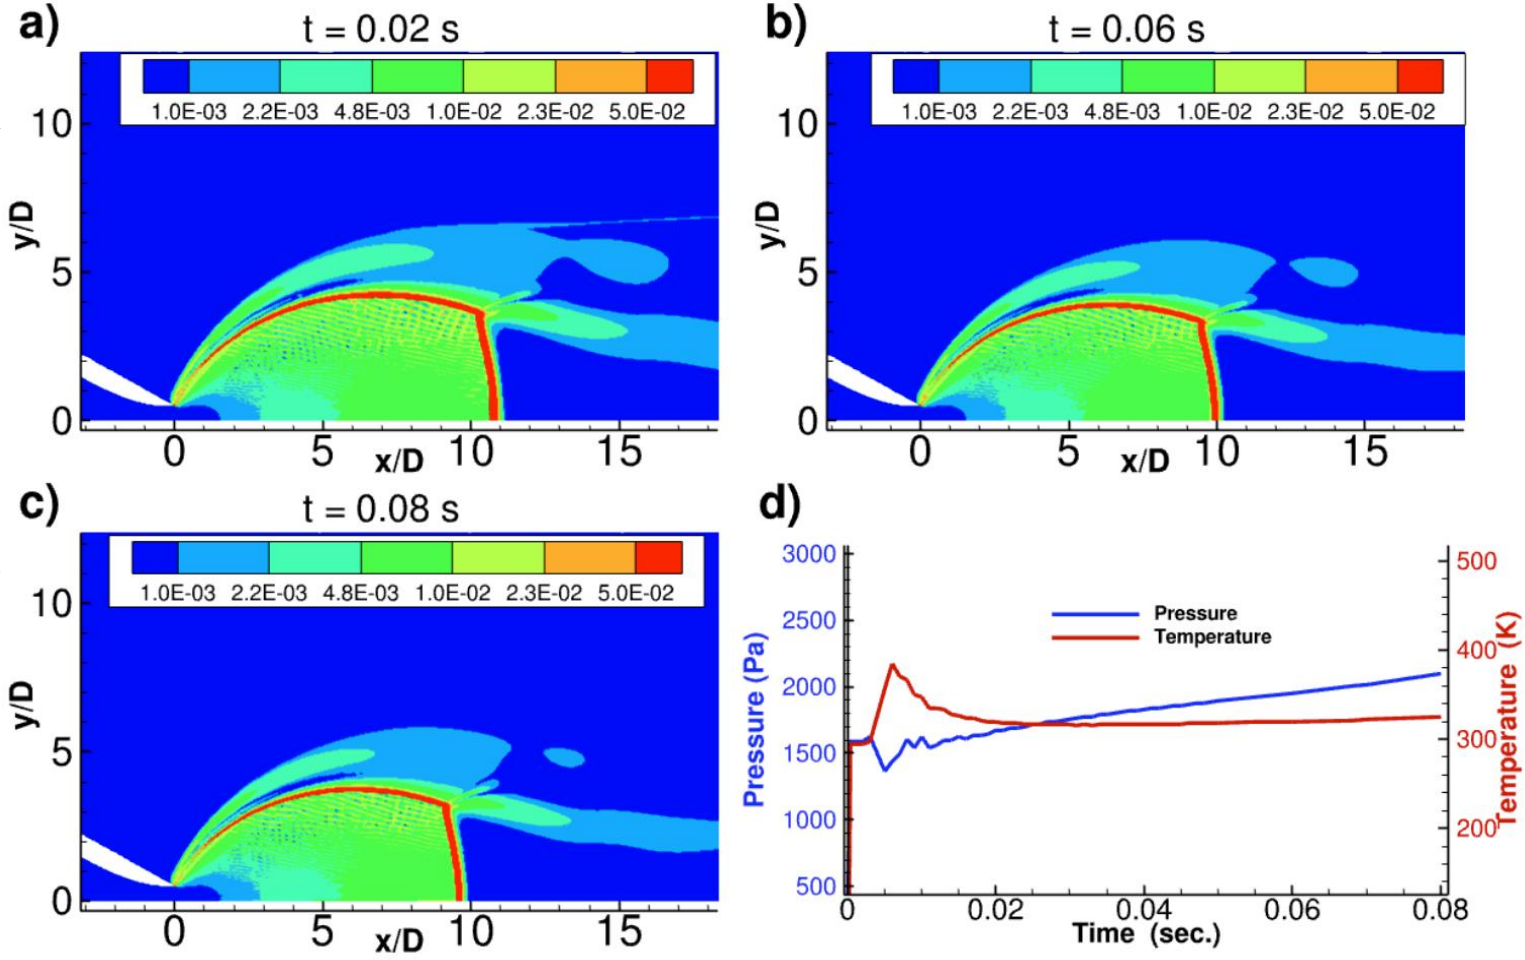
\includegraphics[width=\linewidth]{figs/f16.png}
%    \caption{Temporal evolution of the jet with \hl{NPR=256}. The zero gradient boundary condition allows for the build-up of pressure.}
%    \label{fig:enter-label}
%\end{figure}

%%%%%%%%%%%%%%%%%%%%%%%%%%%%%%%%%%%%%%%%%%%%
\section{Conclusions}\label{sec:conclusions}
%%%%%%%%%%%%%%%%%%%%%%%%%%%%%%%%%%%%%%%%%%%%
With the intent of validating and build trust on the results obtained by the available numerical solvers, Fluent and OpenFOAM, for the Charon (and Eris) jet-ON configuration, additional test cases have been proposed and numerically investigated in the present report. In particular, the dynamics of jet expansion across a spectrum of nozzle pressure and temperature ratios was simulated.
NPR=4.03, NTR=1.0 are presented. Experimental data is available in~\cite{henderson2005experimental} as well as numerical solution from an independent source\footnote{Private communication with Dr. Ozgur Tumuklu (tumuko@rpi.edu). Material avaialble from:~\url{https://www.havalab.org/publications/TumukluAviation2024Jetv2Final.pdf}}.

Numerical validation considered (magnitude) velocity, Mach, static temperature and pressure, and turbulent kinetic energy (TKE) fields. The numerical results obtained with Fluent and OpenFOAM were compared with other numerical solutions and available experimental data.

The obtained numerical results shown a good qualitative and quantitative level of agreement between the two solvers. Fluent solutions appear to be in slightly better agreement with the experimental data.

%%%%%%%%%%%%%%%%%%%%%%%%%%%%%%%%%%%%%%%%%
%\section{Resources}\label{sec:resources}
%%%%%%%%%%%%%%%%%%%%%%%%%%%%%%%%%%%%%%%%%
%
%\begin{itemize}
%    \item \url{https://www.cfd-online.com/Wiki/Codes#Solvers}
%    \item \url{https://arc4cfd.github.io/cfd_codes}
%    \item \url{https://github.com/thw1021/Code4CFD?tab=readme-ov-file}
%\end{itemize}

%%%%%%%%%%%%%%%%%%%%%%%%%%%%%%%%%%%%%%%%%%%%%%%%%%%%%%%%%%
\section{Appendix: post-processing script}\label{sec:post}
%%%%%%%%%%%%%%%%%%%%%%%%%%%%%%%%%%%%%%%%%%%%%%%%%%%%%%%%%%
Listing~\ref{lst:postprocessing} reports a snippet of the script used to post-process the numerical solutions.

\begin{lstlisting}[language=Python,caption={Post-processing script.},label={lst:postprocessing}]
import numpy as np
import pandas as pd
import matplotlib.pyplot as plt
from scipy.interpolate import griddata

d = 0.0126894 * 2 # nozzle diameter

# FLUENT solutions
fluent         = pd.read_csv("../DATA/NPR_4n03_NTR1.csv")
fluent_axis    = fluent[fluent["    y-coordinate"]==0]
planeXY_fluent = pd.read_csv("../DATA/NPR_4n03_NTR1_planeXY.csv")

# EXPERIMENTAL data
expMach = pd.read_csv("../DATA/exp_mach.csv")
expPtot = pd.read_csv("../DATA/exp_tot_press.csv")

# OPENFOAM REF. solutions
numVmag = pd.read_csv("../DATA/VmagNum.csv")

# OPENFOAM my solutions
planeYZ = pd.read_csv("../SIMS/planeYZ.csv")
axis    = planeYZ[planeYZ["Points_1"]==0]

# Plotting Pressure along centerline
plt.plot(axis["Points_0"]/d,axis["p"], 'go', label="OpenFOAM")
plt.plot(fluent_axis["    x-coordinate"]/d,fluent_axis["absolute-pressure"],c='b',label="Fluent")
plt.xlabel("x/D")
plt.ylabel("P (Pa)")
plt.grid()
plt.legend()
plt.savefig("figs/p.pdf")
plt.show()
plt.close()

# Centerline TKE Profile
y   = planeYZ['Points_0']
z   = planeYZ['Points_1']
tke = planeYZ['k']

z_center  = 0
tolerance = 0.05 * d

centerline_mask = (z >= z_center - tolerance) & (z <= z_center + tolerance)
y_center = y[centerline_mask]
tke_center = tke[centerline_mask]

plt.figure(figsize=(10, 4))
plt.scatter(y_center / d, tke_center/(420**2), label='TKE', color='blue')
plt.xlabel(r'x/$D_{jet}$')
plt.ylabel(r'k/$U_{jet}^2$')
plt.title('Turbulent Kinetic Energy vs Streamwise Distance')
plt.grid(True)
plt.tight_layout()
plt.savefig("figs/TKE_vs_xD.pdf")
plt.show()
plt.close()
\end{lstlisting}

% Signature %%%%%%%%%%%%%%%%%%%%%%%%%%%%%%%%%%%%%%%%%%%%%%%%%%%%%%%%%%%%%
\vspace{\fill}
\begin{center}
    \hspace*{9.0cm} \LARGE \textbf{Lorenzo Campoli} \\
    \hspace*{9.0cm}
\includegraphics[width=0.45\textwidth]{
    signature/signature0.png}
\end{center}

\vspace*{-1.0cm}

\hspace*{9.0cm}\textbf{Senior Systems Modelling Engineer}

\hspace*{9.0cm}\textbf{Gilmour Space Technologies}

\hspace*{9.0cm}\textbf{lorenzo.campoli@gspace.com}
%%%%%%%%%%%%%%%%%%%%%%%%%%%%%%%%%%%%%%%%%%%%%%%%%%%%%%%%%%%%%%%%%%%%%%%%%%

\bibliography{refs/refs}
\bibliographystyle{unsrt}

\end{document}